\documentclass[a4paper]{report}
\usepackage{setspace}
%\usepackage{subfigure}

\pagestyle{plain}
\usepackage{amssymb,graphicx,color}
\usepackage{amsfonts}
\usepackage{latexsym}
\usepackage{amsmath}
\usepackage[a4paper, margin = 3cm, bottom = 2.5cm]{geometry}
\usepackage{hyperref}
\usepackage{booktabs}

\usepackage{biblatex}
\usepackage{url}
\usepackage{adjustbox}
\usepackage{listings}
\usepackage{textcomp}
\usepackage{listings}
\usepackage{xcolor}
\usepackage[english]{babel}
\usepackage[utf8]{inputenc}
\usepackage{multirow}  

\usepackage{biblatex}
\addbibresource{bibliography.bib}

%New colors defined below
\definecolor{codegreen}{rgb}{0,0.6,0}
\definecolor{codegray}{rgb}{0.5,0.5,0.5}
\definecolor{codepurple}{rgb}{0.58,0,0.82}
\definecolor{backcolour}{rgb}{0.95,0.95,0.92}

%Code listing style named "mystyle"
\lstdefinestyle{mystyle}{
  backgroundcolor=\color{backcolour},   commentstyle=\color{codegreen},
  keywordstyle=\color{magenta},
  numberstyle=\tiny\color{codegray},
  stringstyle=\color{codepurple},
  basicstyle=\ttfamily\footnotesize,
  breakatwhitespace=false,         
  breaklines=true,                 
  captionpos=b,                    
  keepspaces=true,                 
  numbers=left,                    
  numbersep=5pt,                  
  showspaces=false,                
  showstringspaces=false,
  showtabs=false,                  
  tabsize=2
}

%"mystyle" code listing set
\lstset{style=mystyle}

\newtheorem{theorem}{THEOREM}
\newtheorem{lemma}[theorem]{LEMMA}
\newtheorem{corollary}[theorem]{COROLLARY}
\newtheorem{proposition}[theorem]{PROPOSITION}
\newtheorem{remark}[theorem]{REMARK}
\newtheorem{definition}[theorem]{DEFINITION}
\newtheorem{fact}[theorem]{FACT}

\newtheorem{problem}[theorem]{PROBLEM}
\newtheorem{exercise}[theorem]{EXERCISE}
\def \set#1{\{#1\} }

\newenvironment{proof}{
PROOF:
\begin{quotation}}{
$\Box$ \end{quotation}}

\graphicspath{ {./images/} }

\newcommand{\nats}{\mbox{\( \mathbb N \)}}
\newcommand{\rat}{\mbox{\(\mathbb Q\)}}
\newcommand{\rats}{\mbox{\(\mathbb Q\)}}
\newcommand{\reals}{\mbox{\(\mathbb R\)}}
\newcommand{\ints}{\mbox{\(\mathbb Z\)}}
\newcommand{\code}[1]{\texttt{#1}}

%%%%%%%%%%%%%%%%%%%%%%%%%%


\title{{\vspace{-14em} 
\includegraphics[scale=0.4]{ucl_logo.png}}\\
{{\Huge Hotel Reviews Analyser System Incorporating Sentiment Analysis}}\\
}
\date{Submission date: Day Month Year}
\author{Candidate Number: NSZW1\thanks{
{\bf Disclaimer:}
This report is submitted as part requirement for the BSc Degree in Computer Science at UCL. It is
substantially the result of my own work except where explicitly indicated in the text. The report may be freely copied and distributed provided the source is explicitly acknowledged.}
\\ \\
BSc Computer Science\\ \\
Supervisor: Anthony Hunter}



\begin{document}
 
\onehalfspacing
\maketitle
\begin{abstract}
Over the past few decades, with the increasing use of internet and advancements in online applications, people’s lifestyles have shifted into the new habit of “doing things online”. For travelers and holiday makers, being able to plan out their route and select the appropriate hotels before travelling is crucial in their preparation stage. However, choosing the best hotels can be a daunting task. The amount of information available online may not be accurate, travellers tend to go through the reviews to see what are people's experiences were with this hotel. However, there could be hundreds of reviews for each hotel, and it becomes time consuming to read through each. Thus the system developed in this project will use an opinion-based sentiment analysis to examine the reviews related to every hotel within the database, extracting key information to help users to understand why a particular hotel has been given a good or bad rating. Furthermore, this approach combines lexical analysis, syntax analysis and supervised machine learning algorithms to understand the sentiment of the reviews.

\end{abstract}
\tableofcontents
\setcounter{page}{1}


\chapter{Introduction}
In this chapter, the report will begin by outlining the motivations of this project. Then specify the aims that the system want to achieve, followed by an overview of how the project has been carried out. Lastly, a brief overview of the structure of the rest of the report.

\section{Motivations}
The convenience and variety of public transports available today, has made travelling easy and affordable. Around the globe, demand for good hotels is on a constant rise for the holiday makers and business travellers. Each hotel seeking individual has different needs, it is difficult for a single hotel to cater for all the different features demanded by the travellers. A highly rated hotel may be enjoyed by a group of people, but at the same time disliked by others. In modern hotel booking websites, many indicators and descriptions were given, in order for a regular individual to make a decision on which hotel to choose. Putting aside the destinations, two important factors that tends to be considered the most are the average score of the hotel and the huge number of customer reviews, which are fully loaded with useful information.
\\\\
The average scores given can only provide a general idea as to whether the majority of customers think this hotel is good or bad, specific details as to why they think that way were not inferable. Thus, to understand the strengths and weaknesses of the hotels better, it is necessary to perform text analysis on the customer reviews. However, the vast number of reviews are laborious to go through manually, hence the motivation for this project. This report describes the stages of building a system that performs text analysis on a dataset of customer reviews, extracting the key features and putting together a summary report of the hotels. The reports produced can be used by hotel managers to help them understand what are the area of improvements in the hotel, or what is good about their services. At the same time, the report may also be useful to customers that want to book a hotel, because immediately, they can see a summary of what is the experience of other customers. This enables the potential customer to leverage for themselves if the less desirable aspects of the hotel are endurable, or if the hotel is really attractive to them.

\section{Aims}
The main objective of this project is to use the “Hotel\_Reviews.csv" dataset from the \href{https://www.kaggle.com/jiashenliu/515k-hotel-reviews-data-in-europe}{\textbf{kaggle}} website [1], and  build a system that can generate a report for each hotel, outlining the key findings extracted from both the numerical data such as ratings, and textual data involving user reviews. Thus provide a more detailed insight about each hotel.
\\\\
The system also tries to produce a friendly user interface that is straightforward to use by the users. The user may be able to select any hotel that they are interested in from a list of hotels available in the dataset. When a selection is made, a request for the report about the selected hotel will be sent to the analyser system's server, which in turn has to extract relevant information from the files within the database, to put together a concise report for the user.
\\\\
The system also aims to carry out sentiment analysis on the reviews, to make sure that the positive and negative aspects about the hotel within the report are true. This is also a process of validation, because the system has to validate the supposedly “positive" or “negative" reviews in the dataset against the sentiment analyser of the system. 

\section{Project Overview}
This project can be divided into three parts: Front-end, Back-end and Data Analyser. 

\subsection{Data Analyser}
The Data Analyser is the intelligent part of the system. It incorporates various machine learning algorithms and natural language processing techniques to analyse the user reviews within the original dataset. The main function of the Data Analyser is to breakdown the original dataset into smaller results tables, allowing the back-end server to have quick access to the contents it needs.
\\\\
Another key stage in this component is to perform sentiment analysis on the reviews. This has to be done before the positive and negative feature extractions can take place. The majority of this report will be dedicated to explaining the steps taken and technical implementations of this part of the system.

\subsection{Front-end}
The front-end is a user facing dynamic website that begins by displaying a list of hotels for the users to select from. Once the user has selected a hotel that they wish to see, the site will pass on the request to the back-end server to fetch for the relevant report. The returned results are then rendered in the user's browser.

\subsection{Back-end}
Upon receiving a request from the front-end website, the back-end server will process what the targeted hotel is and goes through different result tables within the database to retrieve a set of relevant data. The data obtained are then passed forward to the front-end and be rendered into the format of a report. 

\section{Overview of report structure}
Chapter 2: a general background of the problem that this project is trying to solve is explained within the context of online hotel bookings. Also a list of tools and development softwares used by this project is presented.
\\\\
Chapter 3: the report will start by introducing the architecture of this hotel review analyser system. More detailed implementations of the other components in the system are also explained.
\\\\
Chapter 4: this chapter focuses on the testing results and evaluation of the methods used in the development stages. Especially the performance comparison between various machine learning algorithms.
\\\\
Chapter 5: a summary of the achievements and challenges faced are discussed.

\chapter{Context}
One of the early versions of a hotel recommender system is to take simple averages of all the user ratings associated with each hotel. However, the shortcomings of this method is that only hotels with ratings close to 5-stars, which could be very expensive in the first place, are always ranked first. This results in less variations and other hotels which may be more suited to the user are being pushed to the back, because the recommender system automatically assumes that users only want 5-star rated hotels. This method is appropriate in making quick suggestions. The overall service provided by these hotels are generally satisfactory. Once the users click into a particular hotel, they can read more about the descriptions of the hotels.
\\\\
However, all the textual information that describes the hotel were carefully drafted by the hotel owners themselves, which are subjective and biased towards the good aspects about the hotel. In order to get a full picture of whether the hotel is good or not, users had to read the reviews provided by other customers who have been to the hotel. Their experiences are more useful and less biased than the official descriptions. Therefore, this system will perform text analysis on all the reviews of each hotel, and summarise the key findings into a short report format that is more objective and fair.
\\\\
There is a need for this type of review analysing system because for every hotel on the booking platforms, there could be hundreds of different reviews. It takes time and effort for any person to read through each review about a hotel and make a conclusion on what they think are the best and worst features. The difficulty of this task increases with more hotels joining the booking platform, which is unfit for humans to manually process them. However, this is a perfect task for machines. First of all the reviews were written in English, the wordings will therefore be written in a way that abide by the English grammars. Secondly, some reviews may be repetitive because the reviewers may have shared similar experiences during their stay. Thirdly there already exist a vast number of reviews online and new reviews are constantly generated. These three characteristics about hotel reviews has made it a perfect problem to be solved by techniques in natural language processing, and provides a large number of training data for machine learning algorithms.

\section{Tools}
Below is a list of software tools and programming languages used in the system:
\begin{itemize}
    \item Python - For main development of system: \url{https://www.python.org/}
    \item HTML - Front-end design: \url{https://html.com/}
    \item Scikit-learn - Python based machine learning library. Used for generating classifiers that predict sentiments: \url{https://scikit-learn.org/stable/}
    \item NLTK - Python based natural language processing toolkit. Used in text analysis, information extraction and preprocessing data: \url{https://www.nltk.org/}
    \item Django - Python based tool for building web applications involving front-end and back-end components: \url{https://www.djangoproject.com/}
\end{itemize}



\chapter{Design and Implementation}
This system is built based on the analysis of the `Hotel\_Reviews.csv' dataset, obtained from the \href{https://www.kaggle.com/jiashenliu/515k-hotel-reviews-data-in-europe}{\textbf{kaggle}} website [1]. According to the uploader, this is a dataset crawled from \url{Booking.com}, where all the data were made publicly available. This dataset is suitable for the development of this project because it contains a combination of numerical and textual data,  which is good for report generation.



\section{System architecture}
This analyser system works by first analysing the numerical and textual data, storing the key findings into different categories of smaller files. The files are then queried by the back-end of the system to extract the relevant information needed for producing the report of the hotels. The textual data from the dataset, mainly the customer reviews, are processed using natural language processing packages. A series of text analysis and feature extractions are performed to obtain the key aspects of the hotel that is being talked about in the review. For each hotel, the system is aiming to summarise a list of its best features, which allows the users to quickly see what are the strong points about this hotel. The reviews are also used for sentiment analysis using machine learning techniques, which helps the system to determine whether each review is truly positive or negative. The high level overview of the hotel analyser system's architecture is shown in Figure~\ref{figure:system_architecture}.

\begin{figure}[h]
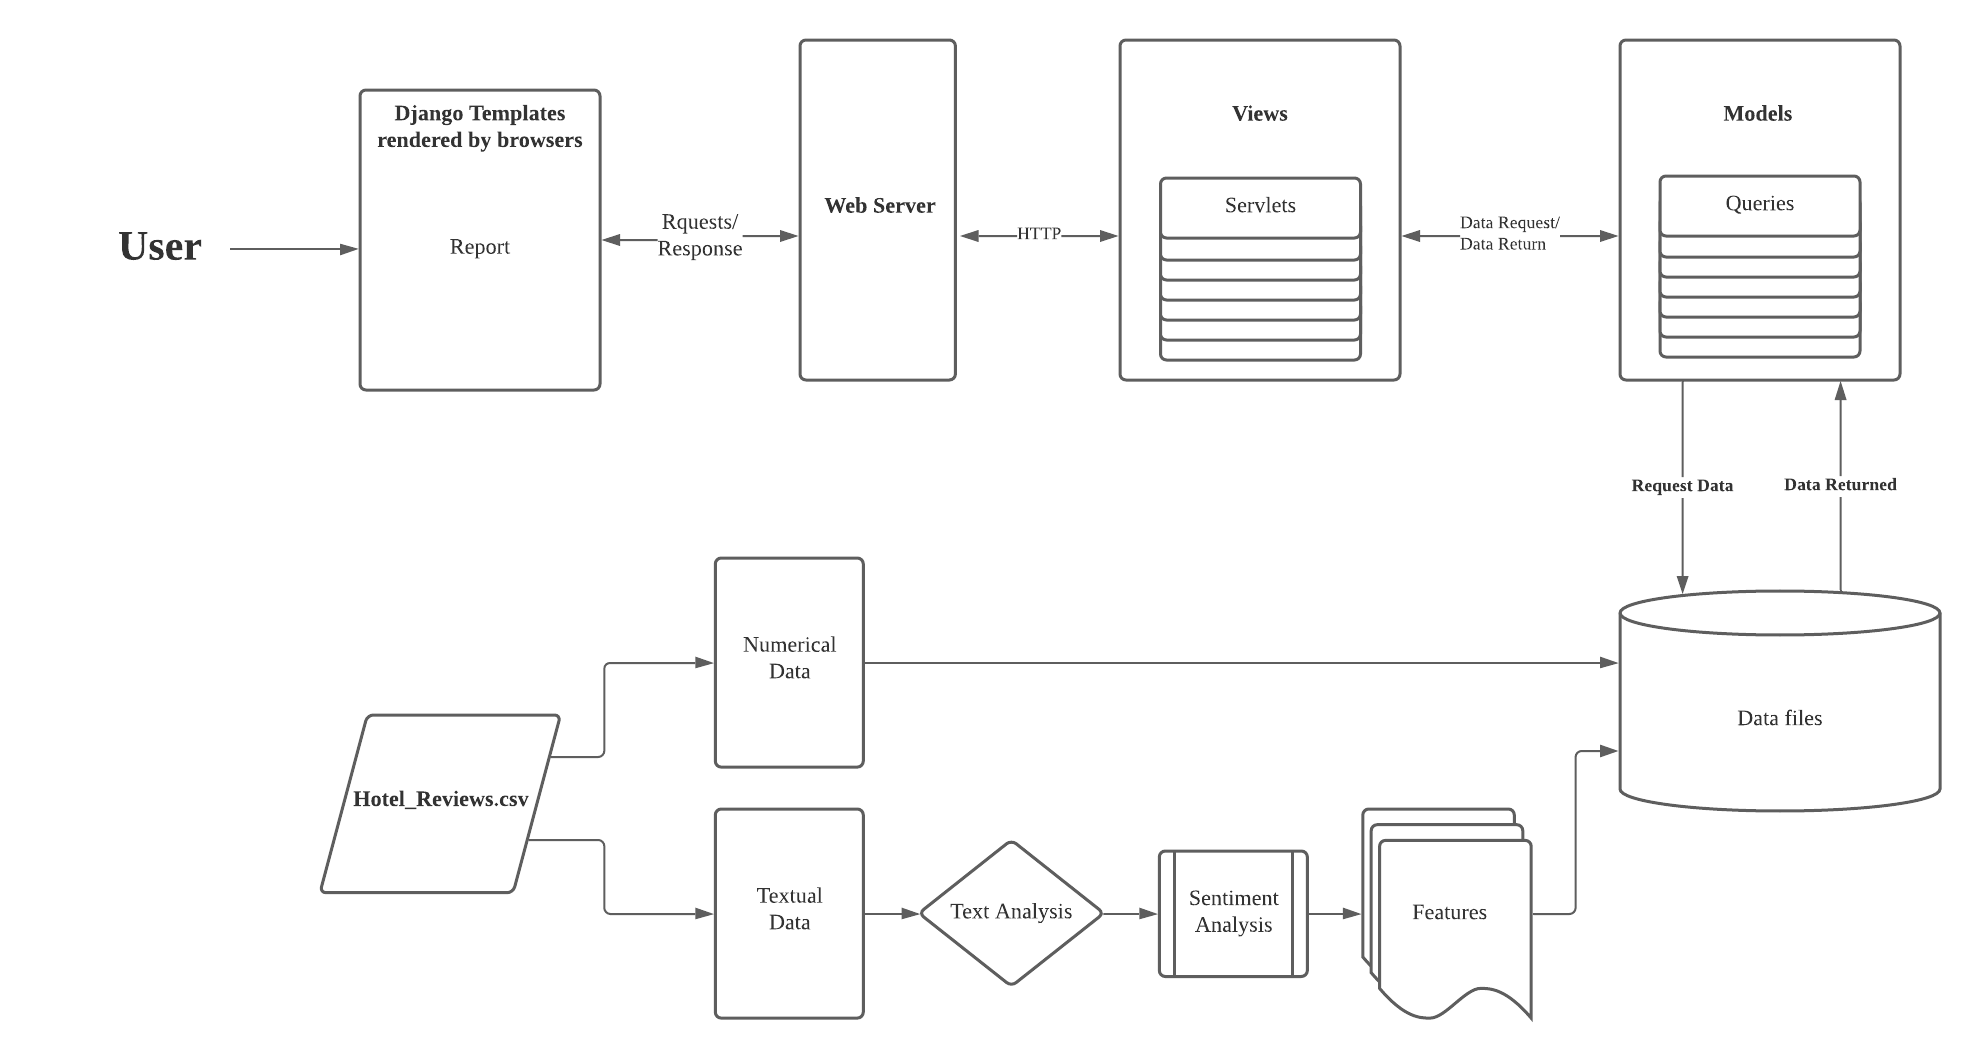
\includegraphics[width=\textwidth, height=7cm, keepaspectratio]{FYP_System Architecture.png}
\centering
\caption{System Architecture}
\label{figure:system_architecture}
\end{figure}

\section{Text analysis}
One of the important aspects in the report produced by this system is to provide a short list of the most liked and disliked features of the target hotel. For each hotel in the dataset, the system examines its corresponding positive and negative reviews and performs feature extraction.
\\\\
In order to extract representative features that are meaningful to the users, the reviews were preprocessed using the NLTK (Natural Language Tool Kit). The following steps of text analysis have been carried out:

\begin{enumerate}
  \item Lexical Analysis
  \item Syntactic Analysis
  \item Semantic Analysis
\end{enumerate}

\subsection{Lexical Analysis}
In NLP (Natural Language Processing), lexical analysis is the study of texts at the words level. It examines the lexical meaning of each individual words.  For example, the word "python" is a noun and "pythonic" is an adjective. In other words, lexical analysis is the process of taking a streams of characters as input and generate a list of tokens together with its respective lexical meanings as the output.

\subsubsection{\textit{Tokenisation}}
The text reviews in the `Hotel\_Reviews.csv' dataset have already undergone some degree of preprocessing where all the punctuations have been removed. Each review is given in the form of a single long string where several sentences are concatenated together. The string is tokenised using the NLTK package's \code{nltk.tokenize.word\_tokenize()} function, stored as a list of word tokens. An example of tokenisation is shown in Table~\ref{table:tokenisation}.


\begin{table}[h]
\centering
\begin{tabular}{ | c || c | }
\hline
\text{ Sentence }   &	\text{The room was big enough and the bed is good} \\
\hline
\text{ Tokenised }  &	\text{[`the', `room', `was', `big', `enough', `and', `the', `bed', `is', `good']}\\
\hline
\end{tabular}
\caption{Example of tokenisation.}
\label{table:tokenisation}
\end{table}

\subsubsection{\textit{POS-tagging}}
In order to detect and correct spelling mistakes in the reviews, each token is passed through a statistical spell checker obtained from \href{https://pypi.org/project/pyspellchecker}{pyspellchecker [2]}. The misspelled tokens are replaced with its most likely correct version. After that, the tokens are labelled with their parts of speech, called part-of-speech tagging using the NLTK package's \code{nltk.pos\_tag()} function. This function considers each token's definition and classifies its appropriate POS-tag according to the context. An example of part-of-speech tagging is shown in Table~\ref{table:pos-tag}.

\begin{table}[h]
\centering
\begin{adjustbox}{width=\columnwidth}
\begin{tabular}{ | c || c | }
\hline
\text{ Tokens }   &	\text{The room was big enough and the bed is good} \\
\hline
\text{ POS-tagged }  &	\text{[(`the', `DT'), (`room', `NN'), (`was', `VBD'), (`big', `JJ'), (`enough', `RB'), (`and', `CC'), (`the', `DT'), (`bed', `NN'), (`is', `VBZ'), (`good', `JJ')]}\\
\hline
\end{tabular}
\end{adjustbox}
\caption{Example of part-of-speech tagging.}
\label{table:pos-tag}
\end{table}

\noindent
The implementation of lexical analysis can be found in Code~\ref{lst:lexical}.  The list of POS-tags and its respective meaning is shown in Code~\ref{lst:POS-tag}.

\subsection{Syntactic Analysis}
Syntactic analysis, as the name suggests is focused on the syntactic level of linguistic processing. This process makes use of the tokens that are POS-tagged in the lexical analysis and attempts to group words into short phrases. This is important because short phrases hold more meaning than just single words. In order to understand what is the main subject being talked about in a given review, the extraction of noun phrases becomes the key component that helps with finding the best features of the target hotel and feature extractions for sentiment analysis at a later stage.

\subsubsection{\textit{Chunking}}
The technical term for extracting short phrases are also called chunking, where small group of words from the sentence are taken as``chunks". Therefore, determining which chunks of the sentence are going to be useful becomes a vital problem. This is achieved by parsing the POS-tagged tokens with predefined grammars that incorporates regular expressions. Taking the POS-tagged sentence in Table~\ref{lst:POS-tag} as an example, the aim is to extract chunks such as ``room was big" and ``bed is good", because they are useful for the system to perform feature extractions.

\subsubsection{\textit{Grammar}}
Thus to capture these phrases, the system uses different grammars to try and match the individual word's POS-tags. As seen in Table~\ref{lst:POS-tag}, the words ``room" and ``bed" both have the `NN' tag, which stands for a noun (see Code~\ref{lst:POS-tag}). The words ``was" and ``is" are labelled as `VBD' (past tense verb) and `VBZ' (present tense verb) respectively, followed by ``big" and ``good" which are both `JJ' adjectives. Example of which grammars can capture these POS-tags are shown in Table~\ref{table:grammar_chunking}. The full grammars used by the system can be found in Code~\ref{lst:grammar_chunking}. In a way, chunking has already removed a lot of redundant data from the sentence structure, reducing dimensionality of the data to save computation power. 

\begin{table}[h]
\centering
\begin{adjustbox}{width=\columnwidth}
\begin{tabular}{ | c || c | }
\hline
\text{ Grammar }   &	\text{Chunking} \\
\hline
\text{\textlangle{} NN\textrangle{}\textlangle{}VBD\textrangle{}\textlangle{}JJ\textrangle{}}  &	\text{(`room', `NN'), (`was', `VBD'), (`big', `JJ')}\\
\hline
\text{\textlangle{}NN\textrangle{}\textlangle{}VBZ\textrangle{}\textlangle{}JJ\textrangle{}}  & \text{(`bed', `NN'), (`is', `VBZ'), (`good', `JJ')}\\
\hline
\end{tabular}
\end{adjustbox}
\caption{Example grammars for chunking.}
\label{table:grammar_chunking}
\end{table}

\subsubsection{\textit{Lemmatization}}
In English, there are many words that looks similar which are derived from a single word, called derived words. The word's structure may change depending on its usage and the part of speech which it is in, in a given context. A language that has derived words in its grammar is also called an inflected language. ``In linguistic morphology, inflection (or inflexion) is a process of word formation,[1] in which a word is modified to express different grammatical categories such as tense, case, voice [...] An inflection expresses grammatical categories with affixation (such as prefix, suffix, infix, circumfix, and transfix)" \href{https://en.wikipedia.org/w/index.php?title=Inflection&oldid=1016909335}{[3]}. Thus the derived words in the tokens can be normalised by reducing them back to their root forms. See example in Table~\ref{table:lemmatization}. This system makes use of the NLTK package's \code{nltk.stem.wordnet.WordNetLemmatizer.lemmatize()} function to obtain the root words called lemmas, which are real words that belongs to the English language. An alternative method of normalisation is stemming, in which the reduced root forms might not be real words, thus losing the original meanings. Therefore only lemmatization is being used in this system.

\begin{table}[h]
\centering
\begin{adjustbox}{width=\columnwidth/2}
\begin{tabular}{ | c || c | }
\hline
\text{ Derived words }   &	\text{ Root word} \\
\hline
\text{ rooms }  &	\text{ room }\\
\hline
\text{ room's }  & \text{ room }\\
\hline
\end{tabular}
\end{adjustbox}
\caption{Example of lemmatization.}
\label{table:lemmatization}
\end{table}

\noindent
Lemmatization is only applied after the stream of tokens has been POS-tagged, so that their original POS-tags are not affected by the modification of the words. The normalisation of tokens are also useful in helping with dimensionality reduction other variations of the same lemma can be discarded.

\subsubsection{\textit{Stop words}}
In each review, there are many words which do not have a lot of meaning, such as ``is",  ``was", ``the'', ``are", ``in", they are commonly referred to as stop words in NLP. To further reduce the data sizes, these words are also removed from the chunks extracted previously. Currently, there is not a global standard in defining which words can be enlisted as a stop words because each NLP tasks is different. Hence in this project, the system uses the list of stop words provided by the NLTK package.
\\\\
After going through the lexical and syntactic analysis, the example sentence in Table~\ref{table:tokenisation} is reduced into the format shown in Table~\ref{table:result}.
\\
\begin{table}[h]
\centering
\begin{tabular}{ | c || c |}
\hline
\text{ Sentence }   &	\text{The room was big enough and the bed is good} \\
\hline
\text{ Processed }  &	\text{[(`room', `NN'),(`big', `JJ')], [(`bed', `NN'),(`good', `JJ')]}\\
\hline
\end{tabular}
\caption{Sentence after undergone Lexical and Syntactic analysis.}
\label{table:result}
\end{table}

\subsection{Semantic analysis}
Unlike the lexical and syntactic analysis, which follows a set of standardised procedures to achieve the results, semantic analysis is less constraint in how it proceeds and open to more interpretations. For humans, it is easy to make sense of a sentence because the brains can automatically recognise the meaning of individual words and the context in which they are used in. Machines on the other hand must be trained to understand the meanings of the text, which is the objective of semantic analysis.

\subsubsection{Hotel features extraction}
Building on top of the refined data obtained from the text analysis stages, the system is able to extract more meaningful data from the reviews, in particular the most liked and disliked features relating to the target hotel.
\\\\
\textbf{\textit{Positive features}}: Given a target hotel, its positive reviews from the dataset were fed into the the text analyser. For each review, a list of refined ``chunks" were extracted. Because of the way that the grammars were defined in Code~\ref{lst:grammar_chunking}, each chunk is a noun phrase. The noun is then taken as the feature with the other values stored under it as a list, forming a feature-value pair. An example output of the semantic analyser is shown in Table~\ref{table:semantic_result}.
\\
\begin{table}[h]
\centering
\begin{tabular}{ | c || c |}
\hline
\textbf{ Feature }   &	\textbf{ Values } \\
\hline
\text{ room }  &	\text{ [`big', `clean', `nice'] }\\
\hline
\text{ bed }  &	\text{ [`good', `comfortable', `large'] }\\
\hline
\text{ staff } & \text{ [`friendly', `helpful', `nice'] }\\
\hline
\end{tabular}
\caption{Semantic analysis output.}
\label{table:semantic_result}
\end{table}

\noindent
After examining each review, the values that correspond to the same features are merged together. The features are then ranked based on the number of values it has. In other words, the features that have been mentioned the most are higher ranked. Later on in the report generation stage, the top 5 features are presented. This is based on the assumption that reviewers tend to comment on the features that they genuinely liked or enjoyed. If something is mentioned more often by a collective, it infers that the hotel has done well in that particular aspect.
\\\\
\textbf{\textit{Negative features}}: The same procedures are also applied to the negative reviews to extract the top 5 most disliked features about the hotel. This is shown as potential areas of improvement for the hotel.



\section{Sentiment analysis}
Sentiment analysis is a sub branch of NLP. It is also called opinion mining, a process to determine whether a piece of text is positive, negative or neutral. This is beneficial to businesses because they could be interested in knowing what is the sentiment of the customer feedback on their products. 

\subsection{Motivation}
For this project, it may first seem that sentiment analysis is not necessary, because the reviews are already classified into positive and negative columns. However, after close examination of the reviews, it turns out that when writing long reviews, users have a high tendency to provide a mixed feedback. For example in a negative review, the user also mentions something good about the hotel. This will affect the best feature selection process previously because the values captured within the ``chunks" may not strictly be positive or negative. Hence the motivation for using sentiment analysis. Each sentence within the review will be passed into the sentiment classifier and be put into positive or negative columns. This approach mines deeper into the text reviews, making sure that the positive sentences hidden in a negative review is taken out and put into the positive section and vice versa for negative sentences. This reclassifying process reduces the number of mixed sentences and improves the system's ability to select the most liked and disliked features.

\subsection{Supervised machine learning problem}
In order to build a sentiment classifier, the system has to be trained using Machine Learning (ML). The main tool used for this section is the Scikit-learn package, which provides many different tools for solving ML related problems. Before diving into the detailed implementations it is important to understand the type of problem at hand so that the appropriate algorithms can be used.
\\\\
The duty of the sentiment analyser is to assign ``positive" or ``negative" labels to the reviews. This is a binary classification problem, a sub-field of supervised ML problem, which requires the training samples to be labelled so that the ML algorithm can produce a model that maps the new reviews to a particular label.

\subsection{Feature extraction}
One of the key aspect in producing reliable ML models that generalises well on unseen data is the quality of the training samples. Unlike numerical data, textual data cannot be analysed by ML algorithms directly, they need to be converted to some sort of numerical representation first. To begin the process, the list of values obtained from the semantic analyser stage (such as in Table~\ref{table:semantic_result}) are used as the base input. The results obtained from text analysis are appropriate because they have already undergone many layers of cleaning. Irrelevant words such as the stop words and even the supposedly good and bad features which are just nouns are discarded. The values left are the key words which by themselves generally reflect a certain sentiment. For example, values such as ``nice", ``friendly" and ``helpful" are words with positive sentiment.

\subsubsection{Bag of words}
A common approach in transforming textual data into a numerical representation is by using bag-of-words (BOW). The list of ``values" or tokens from every chunk are combined into a single feature vector. Then from this feature vector, the number of times each token appears in each review is counted. This produces a document term matrix, where each row is a review (also the document) and each column is the different values (the terms), which is the first numerical representation of the textual data. This is achieved by using the \code{sklearn.feature\_extraction.text.CountVectorizer()} function from the Scikit-learn package. An example of how the document term matrix is generated is shown in Table~\ref{table:document-term-matrix}.
\\\\
Example reviews:
\begin{enumerate}
  \item ``The room was big enough and the bed is good"
  \item ``Comfy bed good location"
  \item ``Bed was extremely comfy"
  \item ``The room is dirty and the windows were broken"
\end{enumerate}

\begin{table}[h]
\centering
\begin{tabular}{ | c || c | c | c | c | c |}
\hline
\textbf{  }   &	\textbf{ big } & \textbf{ good } & \textbf { comfy } & \textbf { dirty } & \textbf { broke } \\
\hline
\textbf{ Review 1 } & \text{ 1 } & \text{ 1 } & \text{ 0 } & \text{ 0 }  & \text{ 0 } \\
\hline
\textbf{ Review 2 } & \text{ 0 } & \text{ 1 } & \text{ 1 } & \text{ 0 }  & \text{ 0 } \\
\hline
\textbf{ Review 3 } & \text{ 0 } & \text{ 0 } & \text{ 1 } & \text{ 0 }  & \text{ 0 } \\
\hline
\textbf{ Review 4 } & \text{ 0 } & \text{ 0 } & \text{ 0 } & \text{ 1 }  & \text{ 1 } \\
\hline
\end{tabular}
\caption{Example of document term matrix derived from the reviews. }
\label{table:document-term-matrix}
\end{table}

\subsubsection{TF-IDF}
For this section, the terms \textit{document} and \textit{review} will be used interchangeably. The bag of words approach works fine for converting text to numbers. However, it has one drawback. It assigns a score to a word based on its occurrence in a particular document, but it does not take into account the fact that the word might also be having a high frequency of occurrence in other documents. TF-IDF resolves this issue by multiplying the term frequency of a word by the inverse document frequency. The TF stands for “Term Frequency" while IDF stands for ”Inverse Document Frequency". It weighs the importance of words in a document, ``then documents with similar, relevant words will have similar vectors, which is what we are looking for in a machine learning algorithm."\href{https://monkeylearn.com/blog/what-is-tf-idf/#:~:text=TF%2DIDF%20enables%20us%20to,in%20a%20machine%20learning%20algorithm.}{[4]}
\\\\
In this project, the TF-IDF is used to help with feature extraction. Words with high TF-IDF scores will be extracted to form feature vectors that helps the ML algorithms to learn how to classify positive and negative sentiments.
\\\\
Notations:
\begin{itemize}
  \item \(t\) is the given term in a document.
  \item \(d\) is a document.
  \item \(n\) is the total number of documents in the document set.
\end{itemize}
\noindent
The Term Frequency is calculated as:
\begin{eqnarray*}
    \begin{aligned}
        tf(t, d) = \log{(1 + f(t, d))}
    \end{aligned}
 \end{eqnarray*}
Here: \(f(t, d)\) is the term frequency in document \(d\).
\\\\
The Inverse Document Frequency is calculated as:
\begin{eqnarray*}
    \begin{aligned}
        idf(t, n) = \log{\left(\frac{1 + n}{1 + df(t)}\right)} + 1
    \end{aligned}
 \end{eqnarray*}
Here: \(df(t)\) is the document frequency of \(t\), which is the number of documents in the document set that contain the term \(t\).
\\\\
The final TF-IDF score is calculated as:
\begin{eqnarray*}
    \begin{aligned}
        tf\text{-}idf(t, d, n) = tf(t, d)*idf(t, n)
    \end{aligned}
 \end{eqnarray*}

\noindent
The implementation of Tf-IDF is shown in Code~\ref{lst:tfidf} .  

\subsection{Training sentiment classifier}
After undergoing the TF-IDF transformation, the document term matrix can be considered as being normalised. The extremely repetitive words are given a lower weight so that their presence in the training data are less dominating over the other word tokens.
\\\\
The normalised document term matrix is now considered as the feature vectors, which will be used as the training dataset. The next step is fed the training set into different ML algorithms that can generate models for binary classification, called classifier. A trained model will be able to classify an input sentence into either the positive sentiment or the negative sentiment categories.
\\\\
The approach adopted in this system is to use not one, but a collective of classifiers that forms a voting system in determining sentiment of sentences. More details on the exact implementations are clearly explained in the next chapter.

\section{Front-end and Back-end}
In order to provide the users of this system with an easy to use interface, this project makes use of the Django web framework that follows a Model-View-Template pattern. The key source code files for implementing this web framework are listed below:

\begin{itemize}
	\item \code{urls.py}
	\item \code{views.py}
	\item \code{models.py}
	\item \code{Templates}
\end{itemize}

\noindent
Figure~\ref{figure:django} illustrates the how a user request is process by the Django system.

\begin{figure}[h]
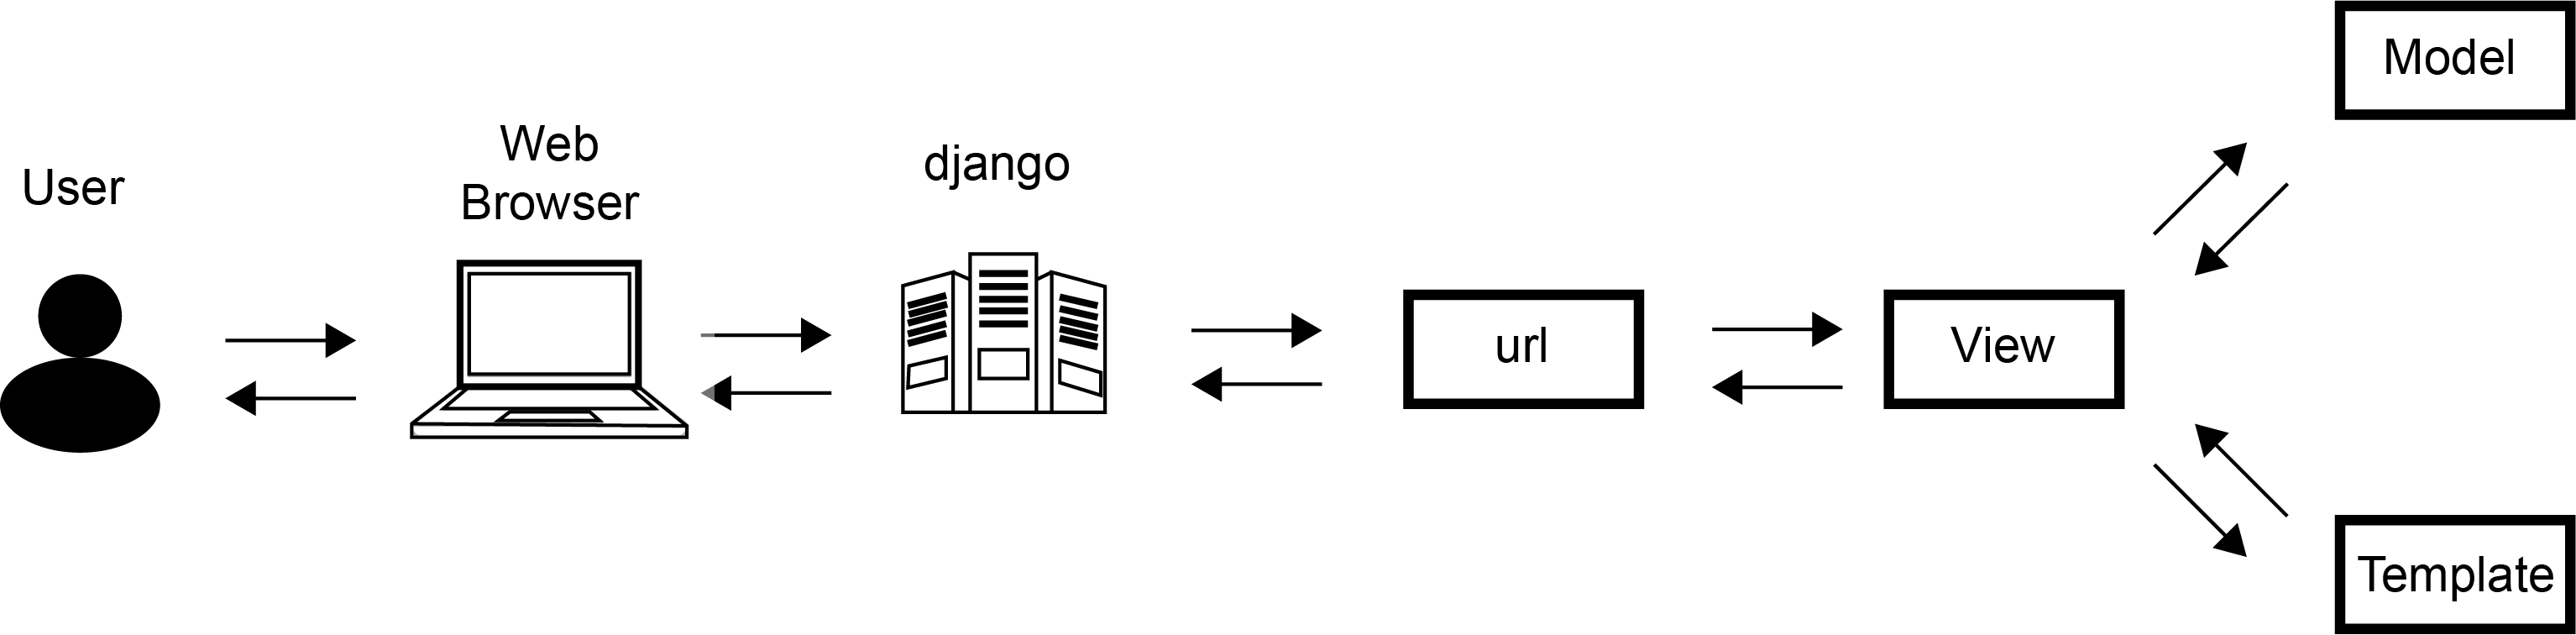
\includegraphics[width=\textwidth, height=7cm, keepaspectratio]{django.png}
\centering
\caption{Django webframework architecture.}
\label{figure:django}
\end{figure}

\subsection{Django web framework}
\subsubsection{urls.py}
This source file is relatively straightforward to follow, it contains a list of allowable URL patterns that joins the various components of the system together. When the Django server receives an incoming request, it checks whether this request is coming from a recognizable website path defined by \code{urls.py}. If the request is valid, the URL pattern will decide which function within the \code{views.py} to call and pass on the requested parameter to that function.

\subsubsection{views.py}
\code{views.py} holds the core functions that can be used by the back-end system. It receives the request and the corresponding parameters, more specifically the name of the hotel requested by the user, from the \code{urls.py} script. In this script, the main function being called will be the \code{report()} function. This is the function for preparing the report because it knows which data is required. However, \code{views.py} does not talk directly to the database, instead, it calls a series of functions in \code{models.py} to fetch the data that it needs. Then it packages up a various data into a Python dictionary and sent it off to a specific template in the \code{Templates} folder.

\subsubsection{models.py}
\code{models.py} acts as the waiter serving the \code{views.report()} function. It receives instruction on which data is needed, then goes through the database files to extract that specific data and passing it back to \code{views.report()}. This is to separate the tasks between the different scripts so that the course codes are more manageable.  

\subsubsection{Templates}
Unlike the first three Python scripts, the \code{Templates} is a folder consisting of \code{.html} scripts. Each \code{.html} script defines the layout of the web page that is going to be rendered in the user's web browser. Namely, \code{report.html} will render the requested report and \code{index.html} will render the home page with the list of hotel names. 
\\\\
After the \code{views.report()} function has acquired the necessary data for a report, it tells the Django \code{controller} that the packaged data should be rendered using the \code{report.html} script. The final rendered report page will be sent back to the user and executed by his or her browser. The reason that the controller's working mechanisms are not discussed in this report is because the controller aspect is managed by the Django framework internally. 

\subsection{User manual}
\begin{enumerate}
	\item In the command line, from the project's home directory, navigate to the \code{Hotel\_report} folder located inside the \code{Django\_Project} folder, which should be the directory containing the \code{manage.py} script.
	\item execute command: \code{python3 manage.py runserver}
	\item Open a web browser and go into \code{http://127.0.0.1:8000/}
\end{enumerate}

\noindent
\textbf{(1)} Having followed the steps above, the browser should boot up the home page as shown in Figure~\ref{figure:user_manual_1}. This displays the list of hotels available from the dataset.

\noindent
\textbf{(2)} Select any hotel available from the list to see the report. Figure~\ref{figure:user_manual_2}.

\noindent
\textbf{(3)} The report includes the following list of information:
\begin{itemize}
	\item Average rating
	\item Location
	\item Nationality of customers who generally enjoyed the stay. This takes the average of all the reviewers from the same nationality.
	\item Nationality of customers who generally disliked the stay.
	\item Best features
	\item Worst features
\end{itemize}

\begin{figure}[h]
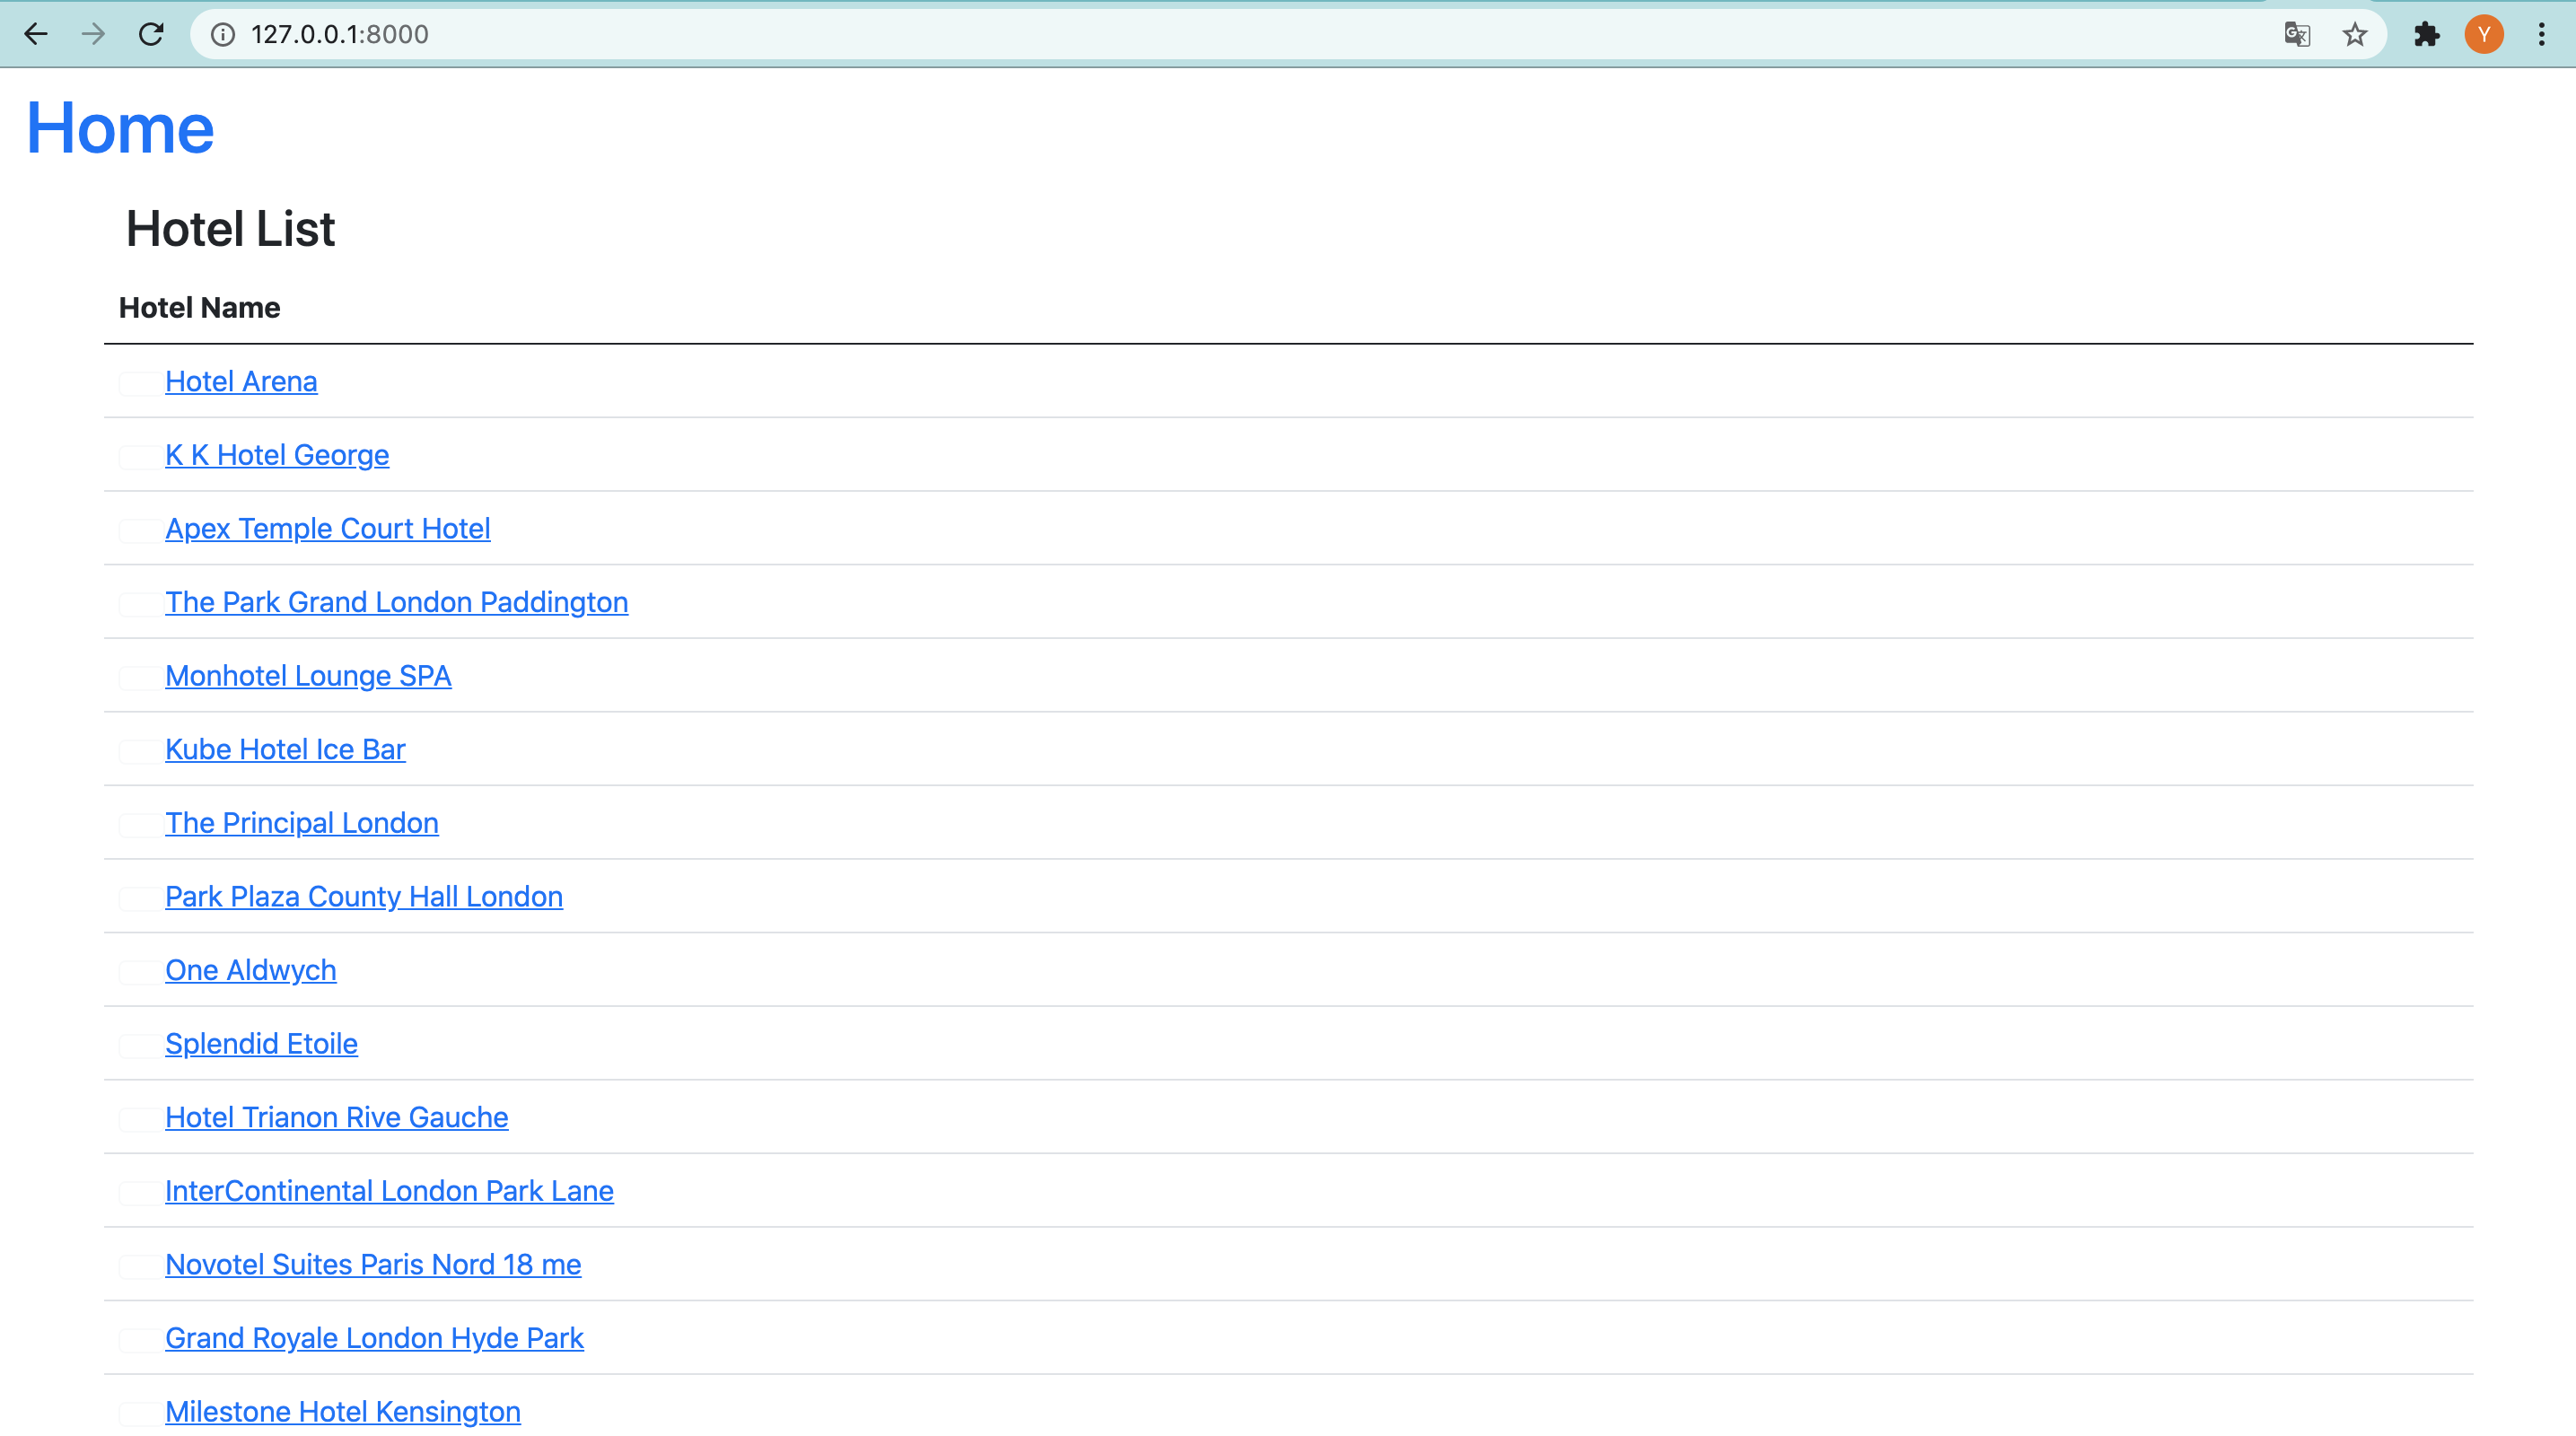
\includegraphics[width=\textwidth, height=7cm, keepaspectratio]{user_manual_1.png}
\centering
\caption{Home page}
\label{figure:user_manual_1}
\end{figure}

{\begin{figure}[h]
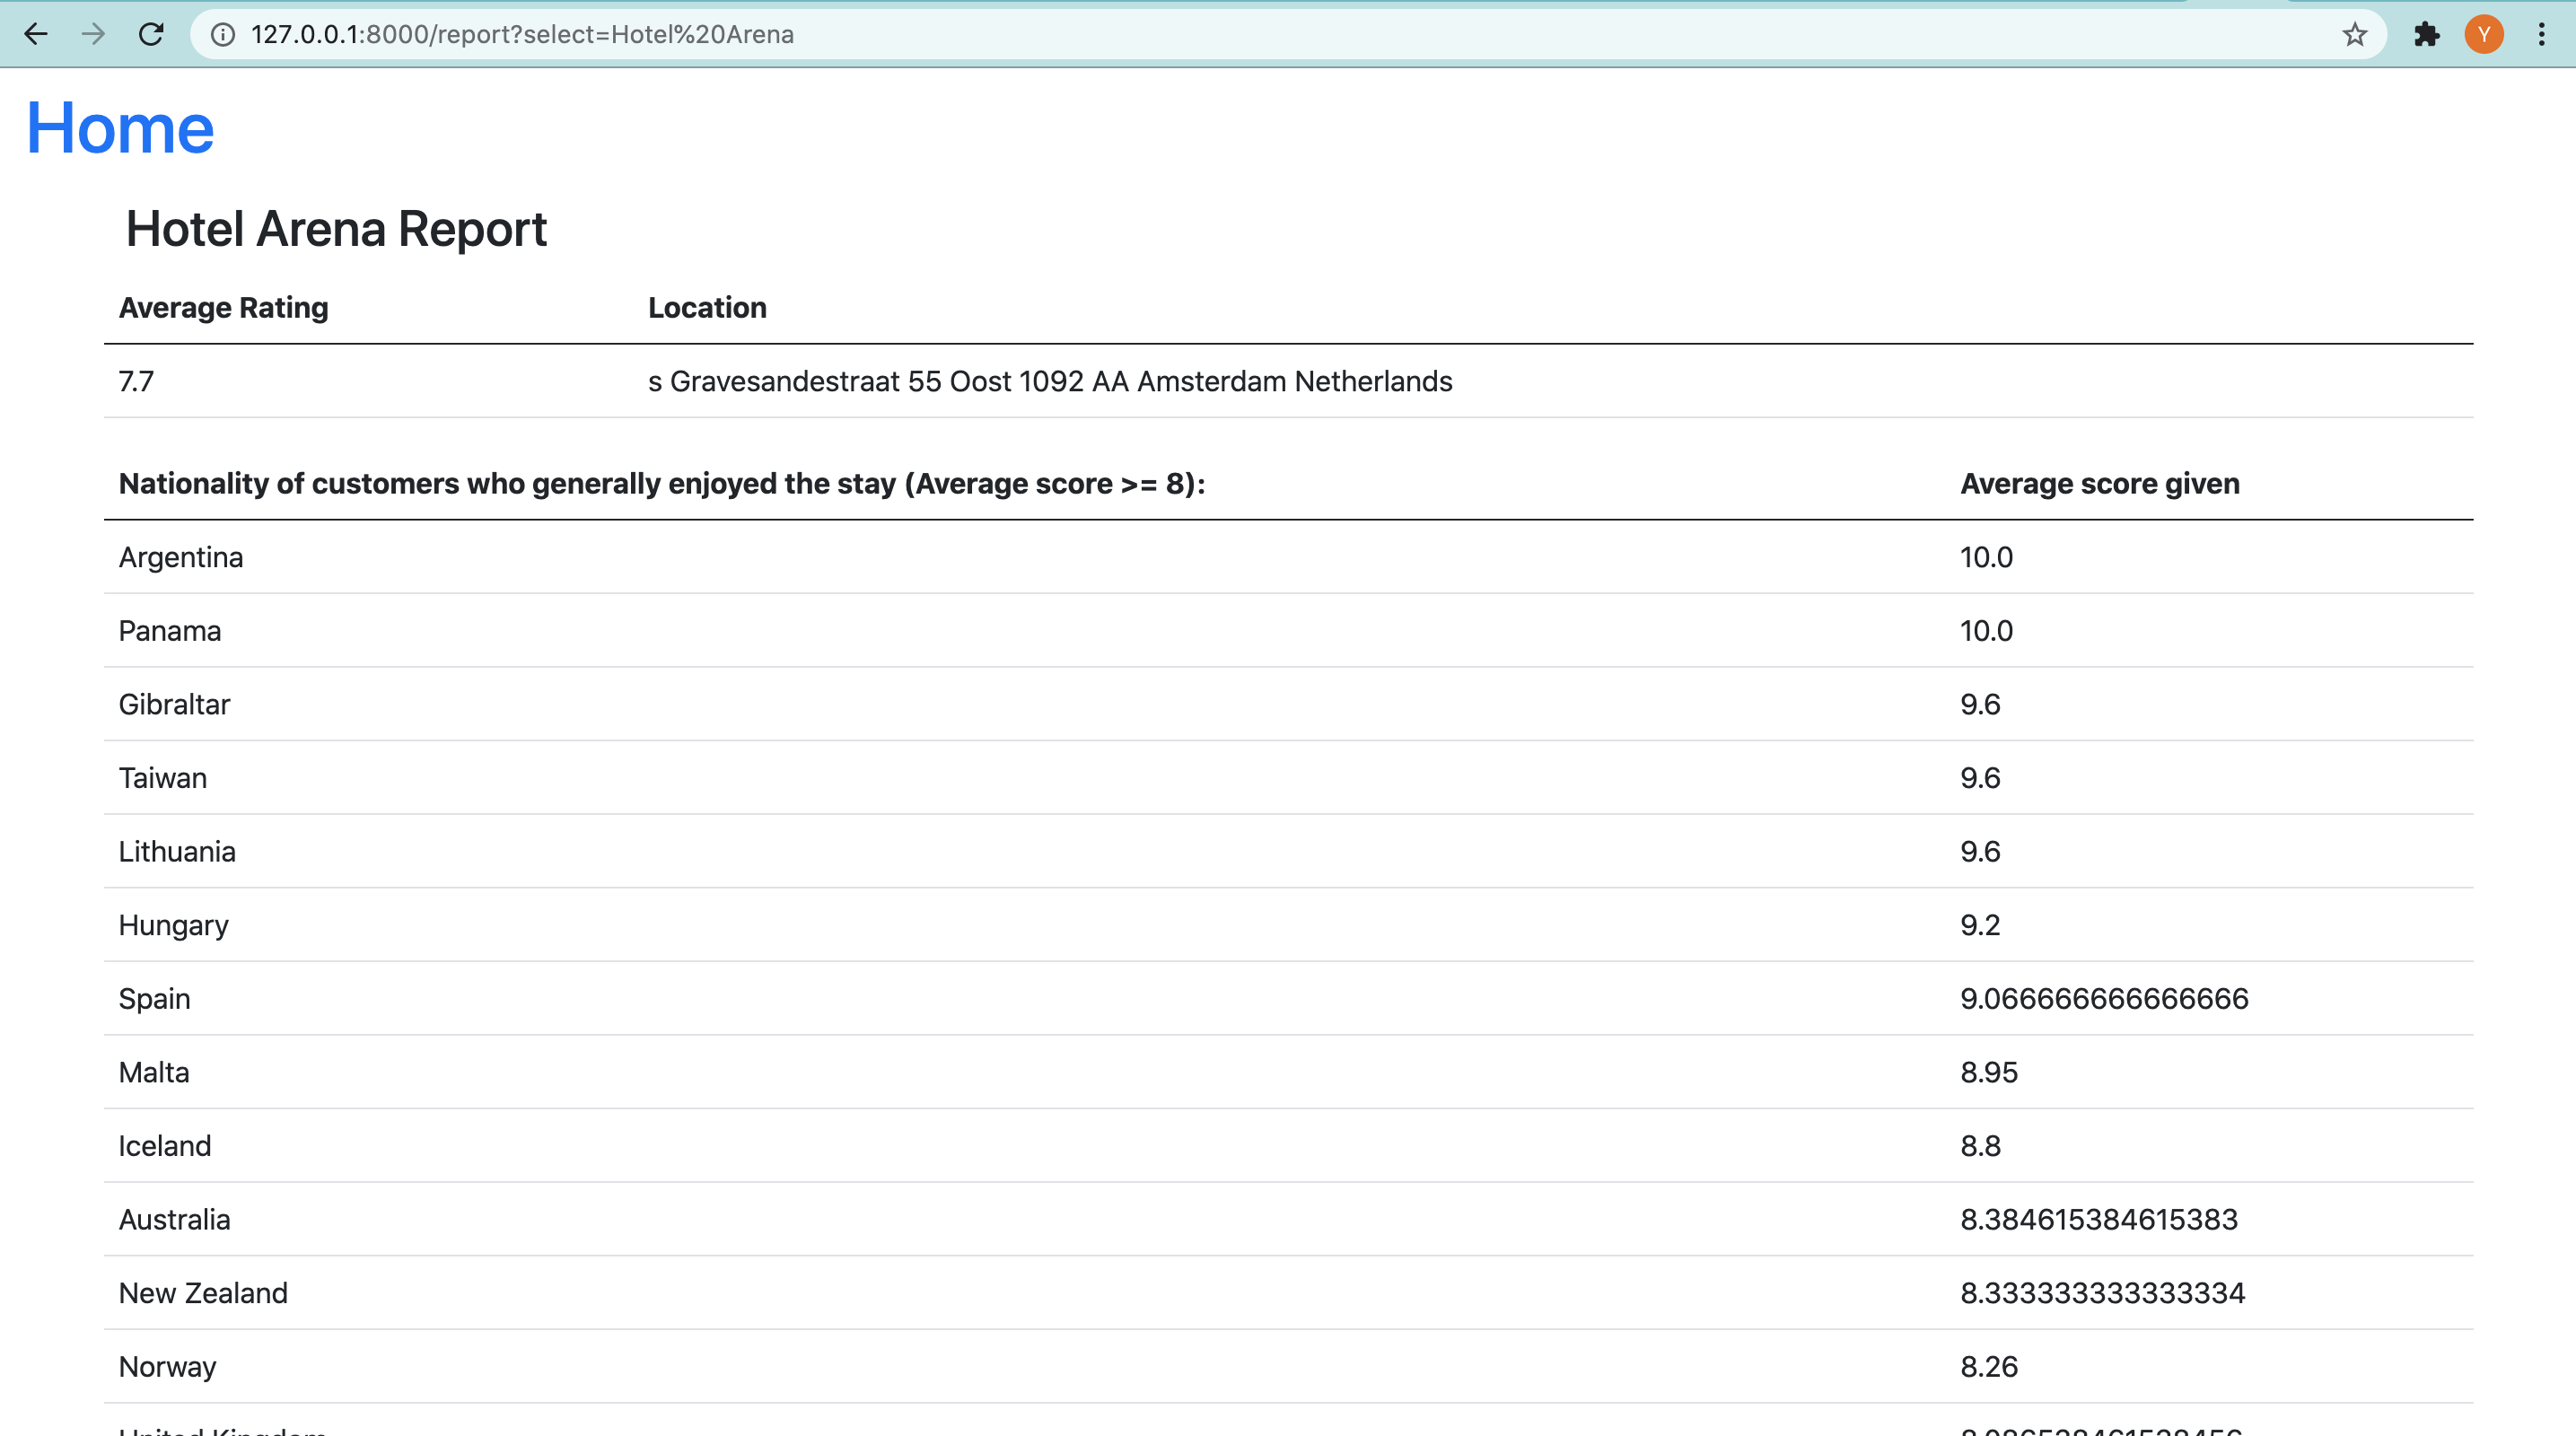
\includegraphics[width=\textwidth, height=7cm, keepaspectratio]{user_manual_2.png}
\centering
\caption{Report page of “Hotel Arena", top section.}
\label{figure:user_manual_2}
\end{figure}

{\begin{figure}[h]
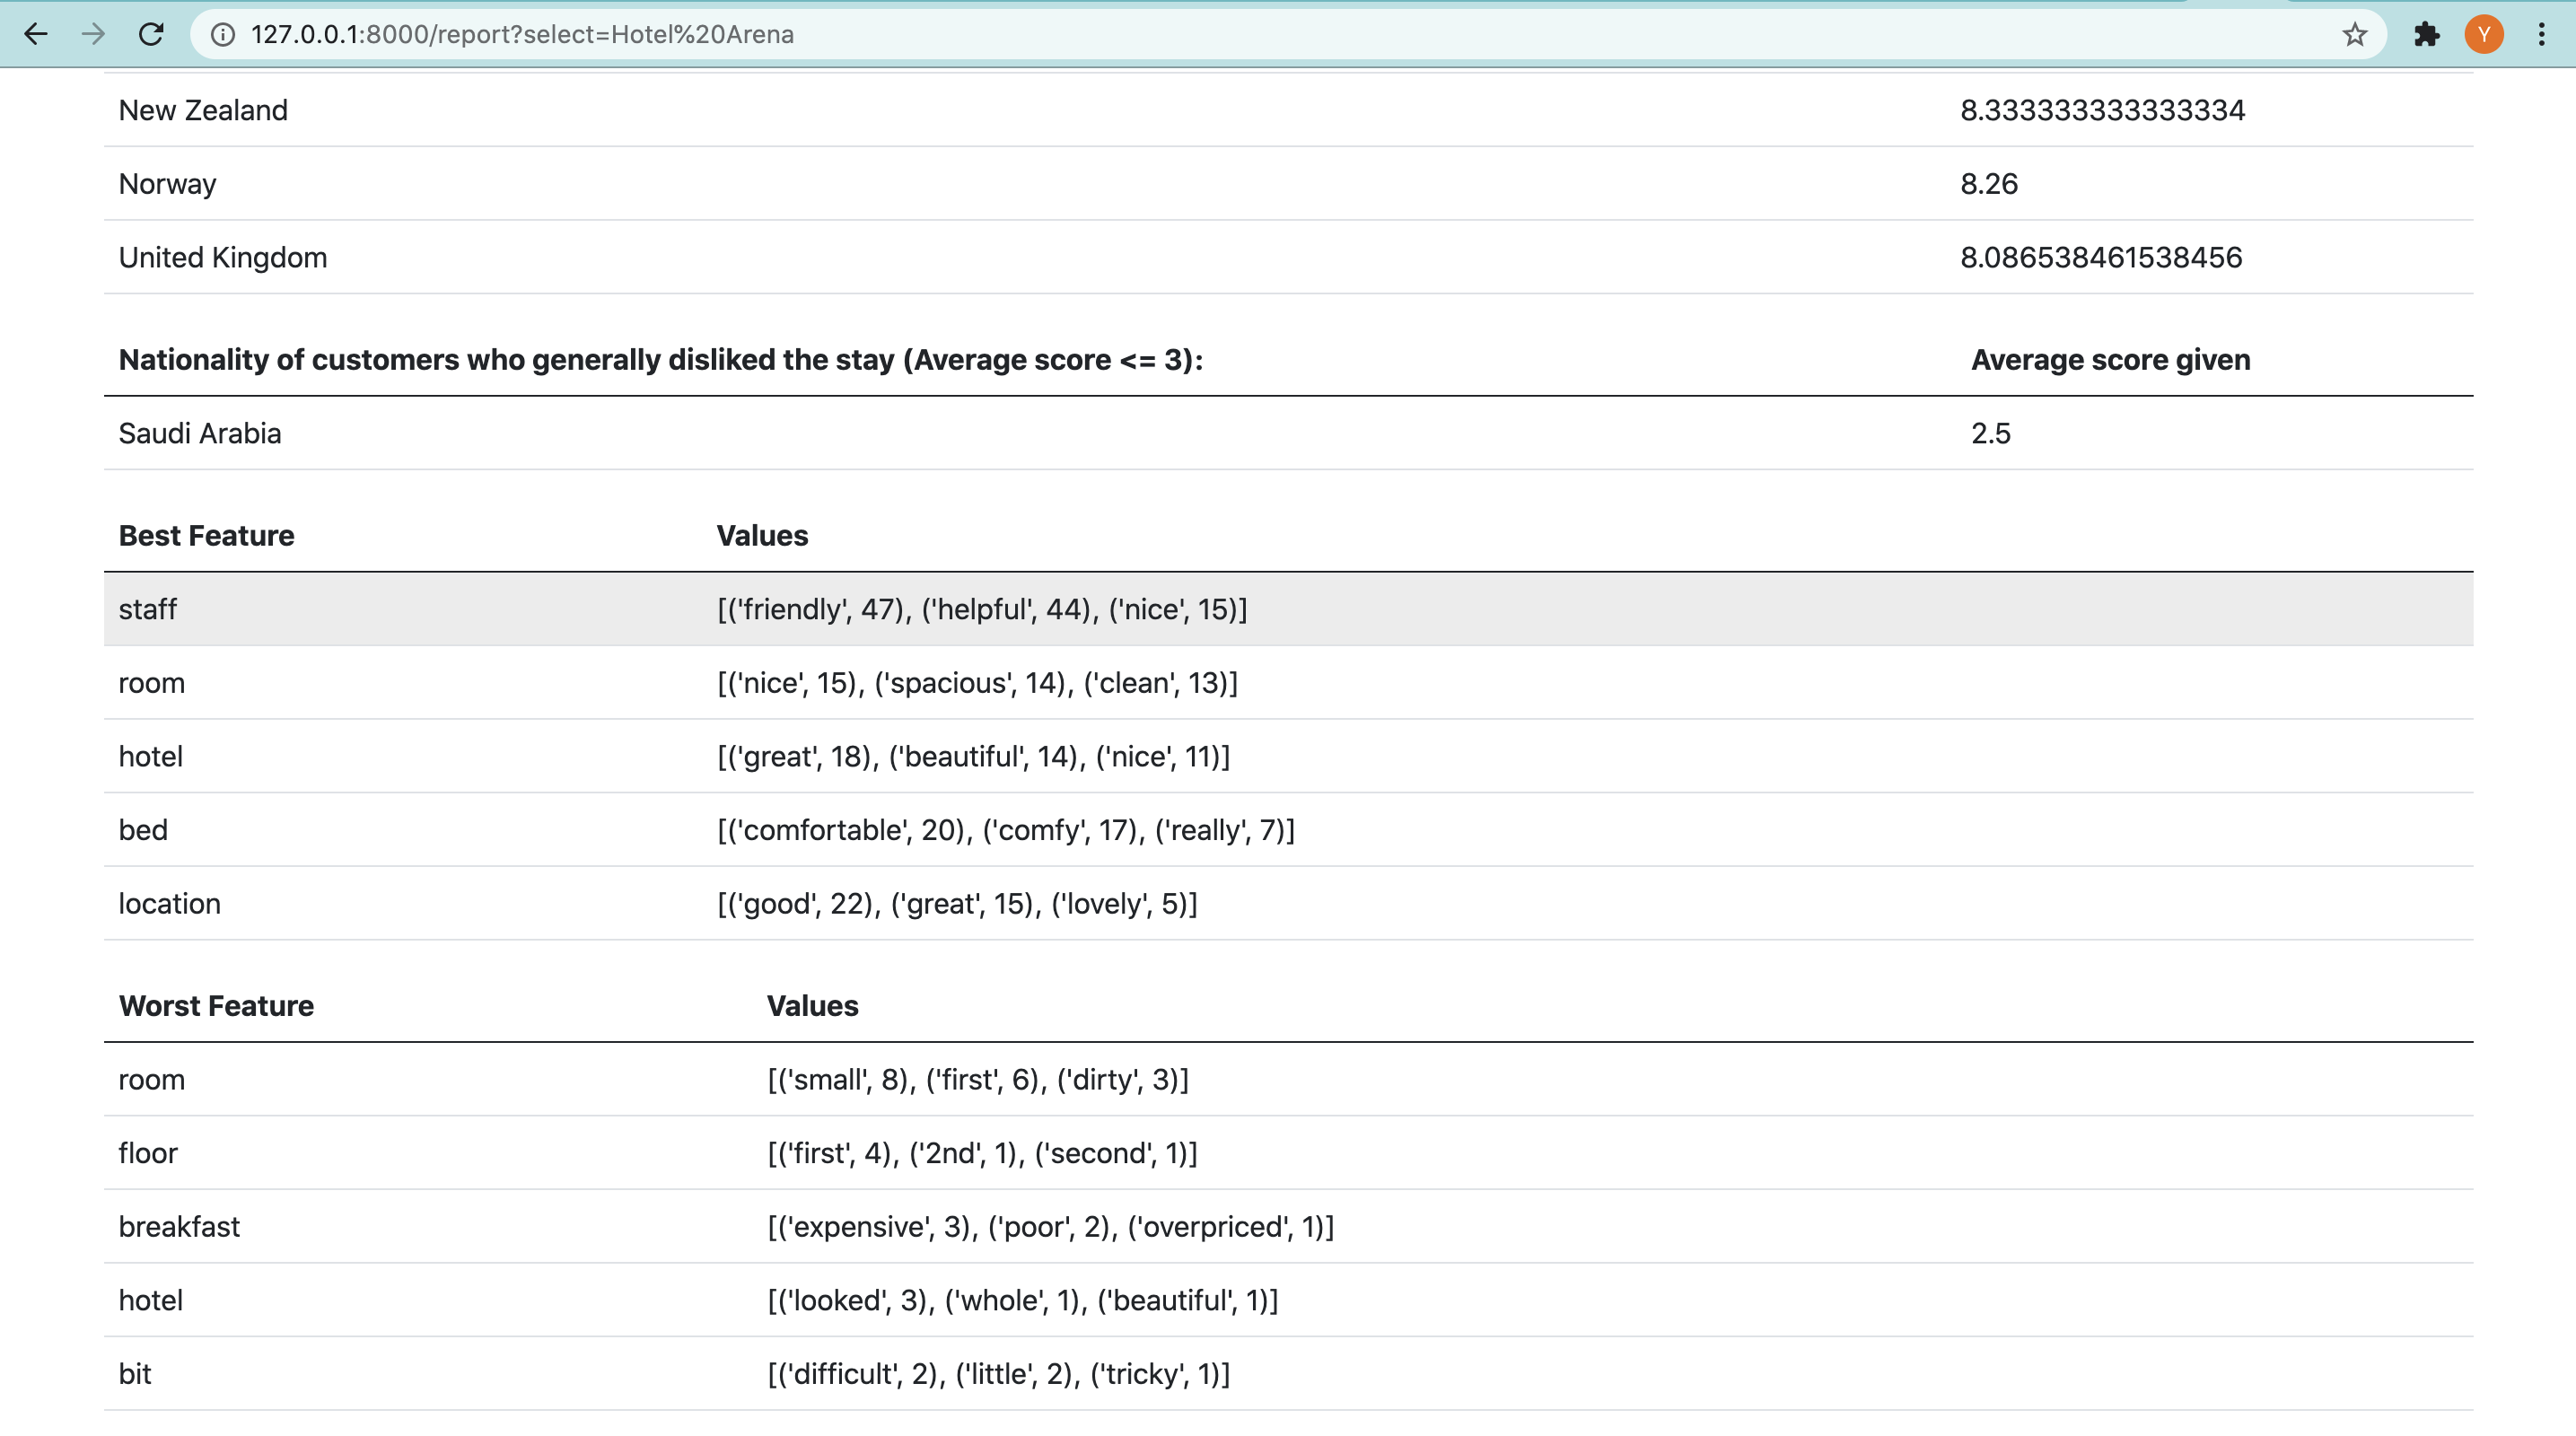
\includegraphics[width=\textwidth, height=7cm, keepaspectratio]{user_manual_3.png}
\centering
\caption{Report page of “Hotel Arena", bottom section.}
\label{figure:user_manual_3}
\end{figure}



\chapter{Testing and Results Evaluation}
Machine learning problems are challenging to solve, the best solution is rarely achieved in the first go. In order to find the best model and its combination of parameters, performance analysis is required. This involves examining the learning curves and compare prediction accuracies to eliminate problems such as overfitting and underfitting. In this chapter, the focus is on how model selection techniques such as cross validation and evaluation metrics are used to help obtain the best sentiment classifier for this system. The main tool used here is the Scikit-learn package. 
The following sections will start by introducing the evaluation metrics used, then move on to the testing of different ML models.

\section{Evaluation metrics}
In order to evaluate the performance of the models, the model's prediction accuracy and the precision and recall values are examined.
\\\\
\textit{Notes:} In the evaluation metrics, the output (0) represents the “negative" label and output of (1) represents the “positive" label.

\subsubsection{Prediction accuracy}
The prediction accuracy is straightforward. This system uses \code{sklearn.metrics.accuracy\_score()} function from the Scikit-learn package to calculate the percentage of the test samples' labels that have been predicted correctly.
\\\\
The equation for accuracy prediction is:
\begin{eqnarray*}
    \begin{aligned}
        \operatorname{accuracy}(y, \hat{y})=\frac{1}{n_{\text {samples }}} \sum_{i=0}^{n_{\text {samples }}-1} 1\left(\hat{y}_{i}=y_{i}\right)
    \end{aligned}
 \end{eqnarray*}
where: \(\hat{y}_{i}\) is the predicted sentiment label of the \(i\text{-}th\) sample and \(y_{i}\) is the true label, \(n_{\text {samples }}\) is the total number of samples tested.
\\\\
\subsubsection{Precision, Recall}
Notations:
\begin{itemize}
	\item \(TP\) stands for True Positive, this is an outcome where the model correctly predicts the positive class.
	\item \(TN\) stands for True Negative, this is an outcome where the model correctly predicts the negative class.
	\item \(FP\) stands for False Positive, an outcome where the model incorrectly predicts the positive class.
	\item \(FN\) stands for False Negative, an outcome where the model incorrectly predicts the negative class.
\end{itemize}

\noindent
\textbf{\textit{Precision}}: This is about calculating what proportion of the positive class predictions are actually correct. The formula of calculation is shown below:
\begin{eqnarray*}
    \begin{aligned}
        \operatorname{Precision}=\frac{TP}{TP + FP}
    \end{aligned}
\end{eqnarray*}

\noindent
\textbf{\textit{Recall}}: This is about calculating what proportion of the actual positive samples are classified correctly. The formula of calculation is shown below:
\begin{eqnarray*}
    \begin{aligned}
        \operatorname{Recall}=\frac{TP}{TP + FN}
    \end{aligned}
\end{eqnarray*}

\noindent
In Table~\ref{table:confusion_matrix} a confusion matrix of the relationships between precision and recall are shown more clearly.

\begin{table}[h]
\centering
\begin{tabular}{ c c c | c | }
& & \multicolumn{2}{c}{Actual label} \\
\cline{3-4}
{} & \multicolumn{1}{ c |} {} & True & False \\
\cline{2-4}
\multirow{2}{*}{Predicted label} & \multicolumn{1}{| c }{True} & \multicolumn{1}{|c|}{True Positive} & False Positive \\
\cline{2-4}
& \multicolumn{1}{|c}{False} & \multicolumn{1}{|c|}{False Negative} & True Negative \\
\cline{2-4}
\end{tabular}
\caption{Confusion matrix.}
\label{table:confusion_matrix}
\end{table}

\noindent
When evaluating the effectiveness of a classifier, precision and recall are examined together. However, in most case, both values are often in competition with each other. Modifying the model to Improve precision may cause recall to decrease and vice versa. But for this system, obtaining a good precision value is slightly more important, because the performance of selecting the best feature and value pairs described earlier, relies on the classifier to have a high confidence in its classifying process.

\subsubsection{F1-score}
The F1-score is another measure of the accuracy performance of a binary classification model. It is defined as the harmonic mean of precision and recall, calculated as follows:

\begin{eqnarray*}
    \begin{aligned}
        \operatorname{F_{1}}=2 \times \frac{\text{precision} \times \text{recall}}{\text{precision} + \text{recall}}
    \end{aligned}
\end{eqnarray*}

\noindent
For instance, a model may have a very high precision with a low recall value, which could give a high accuracy score. It may seem that the model is working well, however in reality, this could be a case of overfitting. Using F1-score, the value calculated will be much lower than the normal accuracy score, because it punishes extreme values in either precision or recall. Thus a high F1-score means a more balanced precision and recall values.

\section{Reasoning of model performance}
The evaluation metrics are very intuitive and straightforward in understanding how well a model has performed. However, that is not the full story, because they are simply the end results. It is essential to be able to understand the reasons that led to these results and finding the flaws in the model. To clarify, this is not about finding flaws in the ML algorithm itself, it is about finding the flaws in the generated model after undergoing training. In particular, there are two main problems faced by a model: underfitting and overfitting.

\subsubsection{Training and testing sets}
The training samples are represented as:
\(\mathcal{S}=\left\{\left(\mathbf{x}^{(i)}, y^{(i)}\right)\right\}_{i=1}^{n}\), where \(\mathbf{x}^{(i)}\) is the feature vector extracted for each review. \(y^{(i)}\) is the label of the corresponding review, which takes the values 0 (negative) or 1 (positive).
\\\\
The entire sample set were then split up with 80\% used as the training set and 20\% used as the testing set. The training set data are used to fit the ML algorithms to generate models. The trained models are then used to predict the mappings on the testing set and evaluation metrics can then be calculated to measure the performance of the model.

\subsubsection{Underfitting}
In simple terms, underfitting, also referred to as high bias, occurs when the model has poor performance on the training set and poor generalization on the test set. This could be due to the model being too simple, it is highly biased towards certain basic assumptions that it fails to capture the other key characteristics of the positive and negative sentiment reviews. This can be overcome by increasing model complexity, enriching its representation of the training data. In other cases, it could also mean that the wrong ML algorithm has been used to generate the model.

\subsubsection{Overfitting}
Overfitting, also referred to as high variance, occurs when the model has good performance on the training set and poor generalization on the test set. This could be due to the model being overly complex, it has tried too hard in learning the key features that appears in each target class in the training set data. This allows a very small room of error. Thus when tested against the previously unseen testing set, data that may have slight differences from what it has seen in training will become unrecognisable for the model and it generalizes poorly on these new data. This can be resolved by reducing the model complexity, taking away subsets of the feature vector that the model uses. Or increase the sample space used in the training process.

\section{Decision Tree Classifier}

The first ML algorithm tested in the development of this analyser system is the Decision Tree Classifier (DTC) algorithm. DTC has a tree structure consisting of nodes and edges, starting from a root node at the top, branching downward to two child nodes. Each node will continue to have two new child nodes until the leaf nodes have been reached. There are two types of nodes, one type is called a decision node, which is used to make a decision in how to split the data. The second type is the leaf node, which represent a final outcome. In this training exercise, the leaf node will represent either “positive" or “negative", because the objective is to determine the sentiment of a sentence after traversing through the series of decision making processes in the tree.

\subsubsection{Criterions for decision node}
At each decision node in the DTC, the algorithm calculates how well a given feature separates the target classes. In the \code{sklearn.tree.DecisionTreeClassifier()} function, there are two criterion available for measuring the quality of split, namely by Gini Impurity and Information Gain. More readings on their working mechanisms can be found \href{https://en.wikipedia.org/wiki/Decision_tree_learning}{\textbf{here}}.

\subsubsection{Tree depth}
Another key parameter which can be configured is the depth of the tree. For a small depth such as 2, the algorithm will converge quickly, because only 3 features will need to be selected before reaching the leaf node. An example tree with depth set to 2 is shown in Figure~\ref{Figure:DTC_depth_2}.
\\
\begin{figure}[h]
\centering
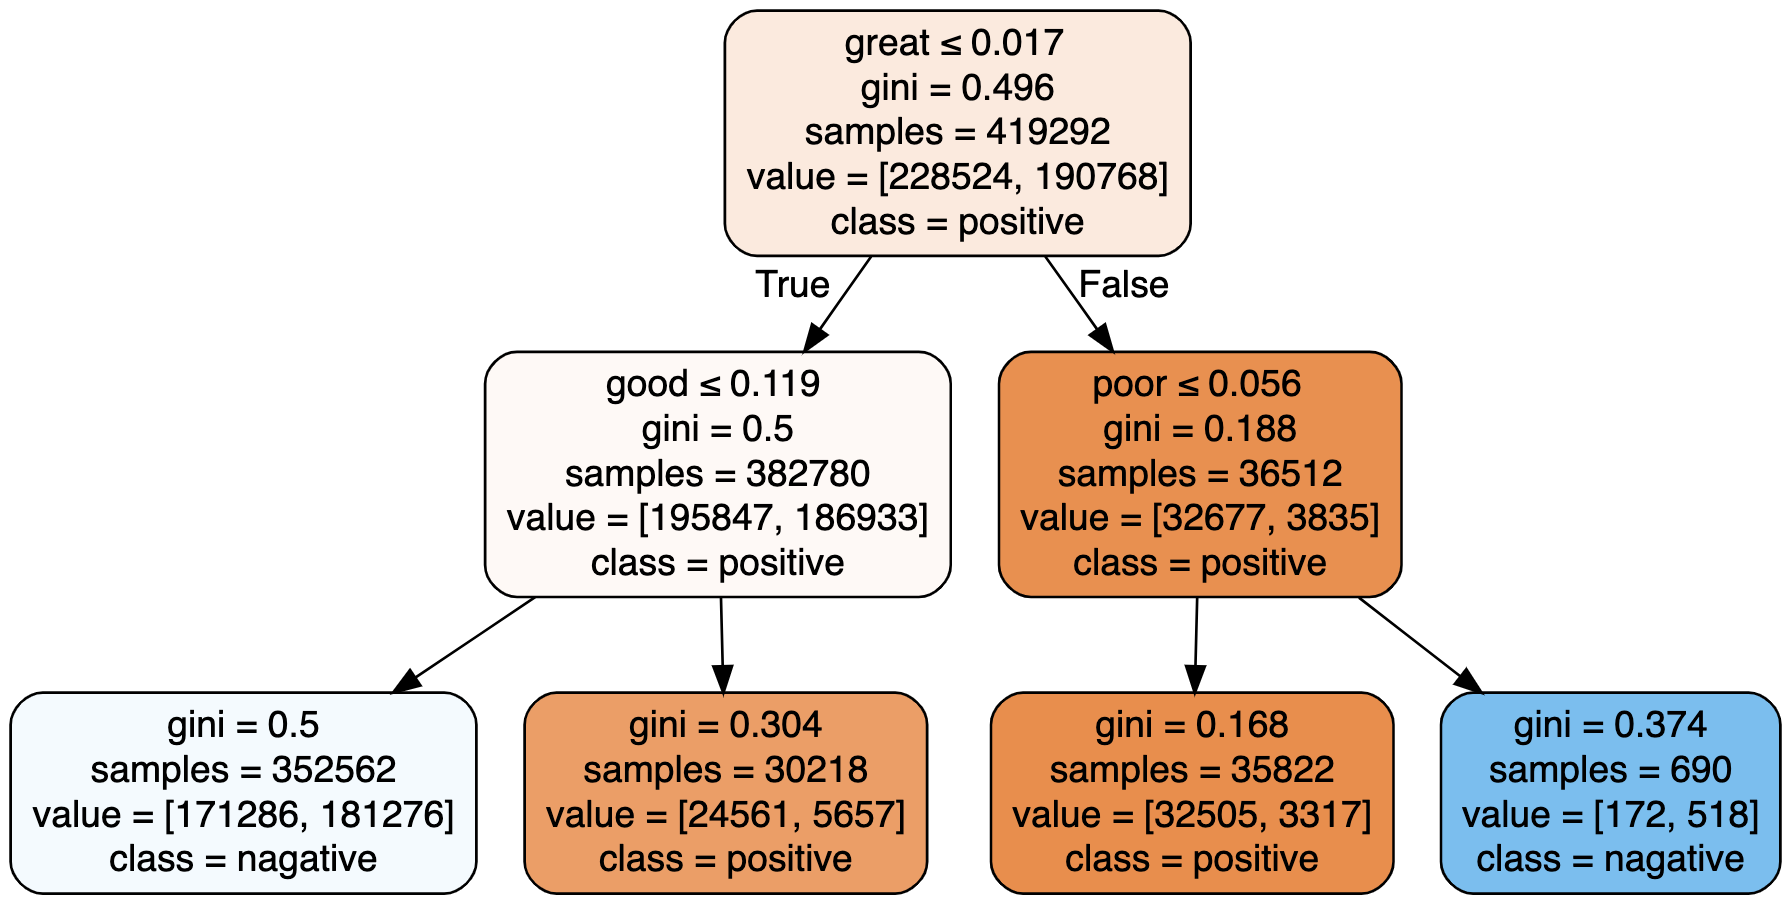
\includegraphics[width=\columnwidth]{Figure_1_DTC_depth_2.png}
\caption{DTC with depths of 2.}
\label{Figure:DTC_depth_2}
\end{figure}

\noindent
As shown in Figure~\ref{Figure:DTC_depth_2}, the root node takes the word “great" as the best feature. It also shows that the term has a higher probability of being labelled as positive. Hence, when predicting the sentiment of a given sentence, DCT first calculates a weighting of the word “great", corresponding to the sentence. If the condition “great \( \leq\) 0.017" is not satisfied, go down to the right branch and check if the condition “poor \(\leq\) 0.056" is satisfied. If the answer is true, then traverse to the left, reaching a positive leaf node.
\\\\
The principle which the DTC follows is therefore very intuitive. The deeper the tree is, the more words will used to from the decision nodes that sits between the root node and the leaf nodes. This will allow the model to capture more variations of the sentence being tested and increase accuracy.

\subsubsection{Testing}
Using the DTC with depth 2 as a starting point, the performance of the model is shown in Table~\ref{table:DTC_depth_2_performance}.
\\

\begin{table}[h]
\centering
\begin{tabular}{  c | c | c | c |}
\cline{2-4}
&  \textbf { precision } &  \textbf  { recall } & \textbf  { f1-score } \\
\hline
\multicolumn{1}{|c|}{\textbf{0}} & 0.51 & 0.95 & 0.67 \\
\hline
\multicolumn{1}{|c|}{\textbf{1}} &  0.87 & 0.25 & 0.39 \\
\hline
\hline
\multicolumn{1}{|c|}{\textbf{Accuracy}} & \multicolumn{3}{|c|}{0.5688446237943963} \\
\hline
\end{tabular}
\caption{Accuracy and Precision Recall of DTC with depth 2.}
\label{table:DTC_depth_2_performance}
\end{table}

\noindent
From the evaluation metrics in Table~\ref{table:DTC_depth_2_performance}, this model has a very high precision in classifying the positive class, so it is confident in choosing which sample has a positive sentiment. But the model also has a low recall, meaning that it tends to miss samples belonging to the positive class, which is why the F1-score is low. Hence the overall accuracy achieved is only around 57\%, not generalizing well on new data.

\subsubsection{Investigating depth}
To remedy this problem, the different depth can be used when training the DTC and choose the depth with the highest accuracy.

\begin{figure}[h]
\centering
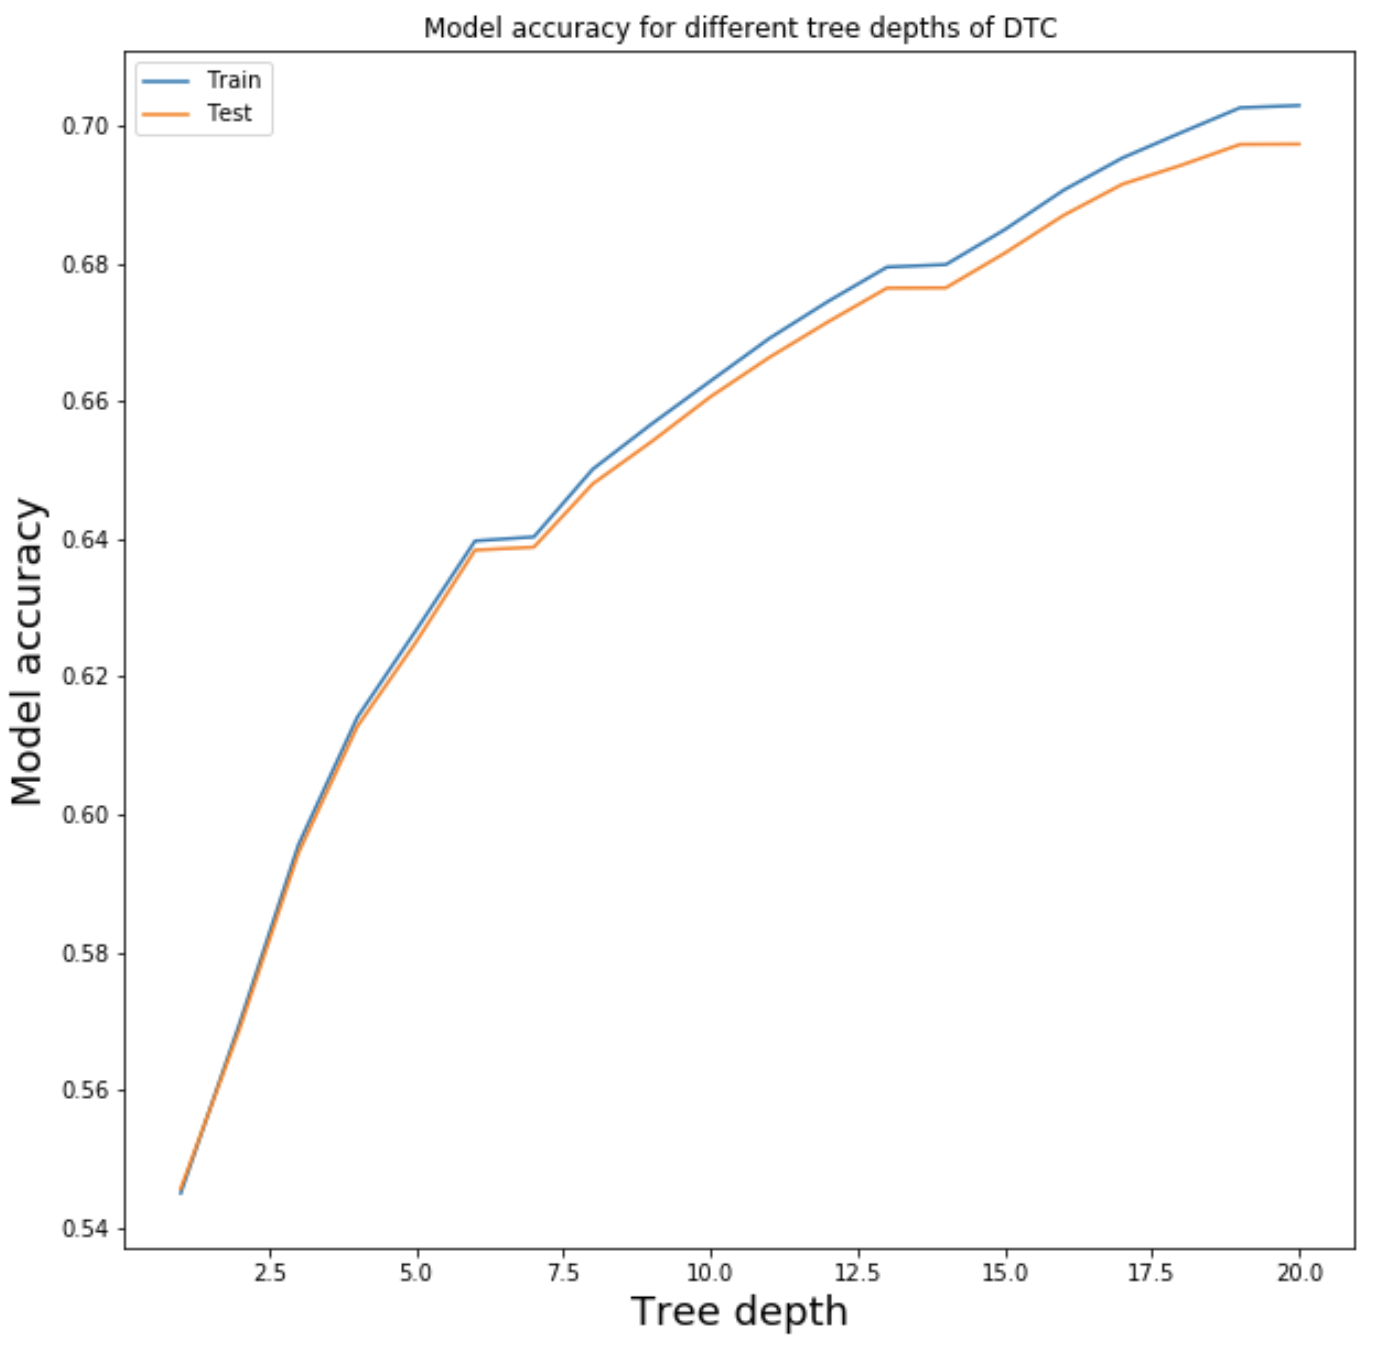
\includegraphics[scale=0.5]{Figure_2_DTC_depths_1_20.png}
\caption{Model accuracy curve.}
\label{Figure:DTC_depth_1_20}
\end{figure}

\noindent
Figure~\ref{Figure:DTC_depth_1_20} shows the accuracy scores of tree depths ranging from 1 to 20. From the graph, as the tree depth used increases, the model's accuracy on classifying both the training and testing set also increases. The exact figures of some of the depths are shown in Table~\ref{table:DTC_accuracy_depth_1-20}.
\\
\begin{table}[h]
\centering
\begin{tabular}{ | c || c | c | c | c | c |}
\hline
\textbf{ Tree depth } & \text{ 1 } & \text{ 5 } & \text{ 10 } & \text{ 15 }  & \text{ 20 } \\
\hline
\textbf{ Accuracy } & \text{ 0.5457} & \text{ 0.6251 } & \text{ 0.6606 } & \text{ 0.6815 }  & \text{ 0.6973 } \\
\hline
\end{tabular}
\caption{DTC prediction accuracies on test set with different tree depths. }
\label{table:DTC_accuracy_depth_1-20}
\end{table}

\begin{table}[h]
\centering
\begin{tabular}{  c | c | c | c |}
\cline{2-4}
&  \textbf { precision } &  \textbf  { recall } & \textbf  { f1-score } \\
\hline
\multicolumn{1}{|c|}{ \textbf {0}} & 0.61 & 0.93 & 0.74 \\
\hline
\multicolumn{1}{|c|}{ \textbf {1}} & 0.90 & 0.50 & 0.64 \\
\hline
\hline
\multicolumn{1}{|c|}{ \textbf {Accuracy}} & \multicolumn{3}{|c|}{0.6973374164067047} \\
\hline
\end{tabular}
\caption{Accuracy and Precision Recall of DTC with depth 20.}
\label{table:DTC_depth_20_performance}
\end{table}

\noindent
At this point, the model generated at depths of 20 shows the best result. The evaluation metrics of this particular model is displayed in Table~\ref{table:DTC_depth_20_performance}. Increasing depth to 20 has improved the model's accuracy by around 15\%. The precision for identifying positive sentiment has now reached 90\%, but the recall value is still a lot lower. Also the precision for identifying negative sentiment is much less than that of positive sentiment. This suggests that the model is only good at identifying the obvious positive sentiment reviews. It's less efficient in understanding the negative sentiments. Therefore more tuning is required.
\\\\
Experiments with other tree depths have been conducted. The accuracy graph for depths values ranging from 20 to 5000 can be found in Figure~\ref{Figure:DTC_depth_20_5000}, Table~\ref{table:DTC_accuracy_depth_20_5000}  has the summary of accuracies.

\begin{figure}[h]
\centering
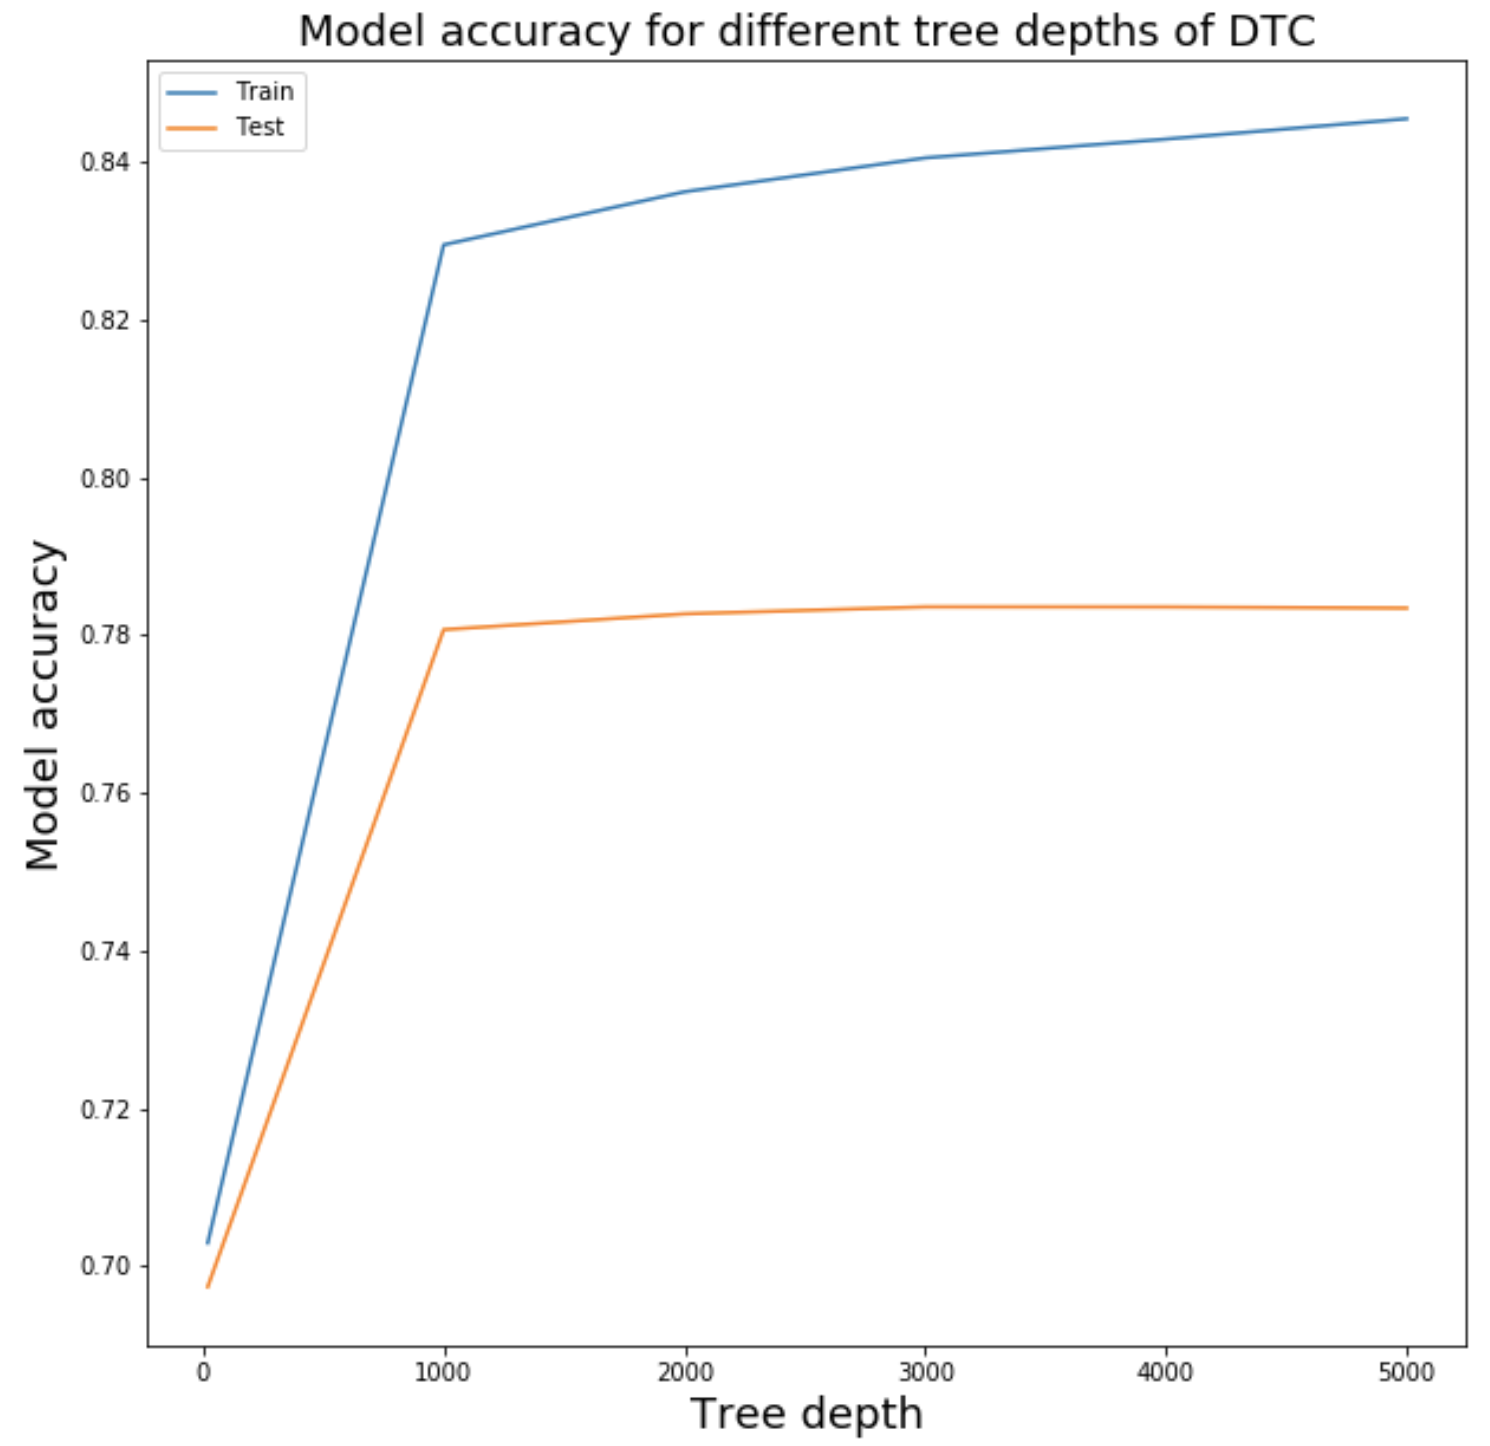
\includegraphics[scale=0.5]{Figure_3_DTC_depths_20_5000.png}
\caption{Model accuracy curve with different depth, using Gini Impurity criterion.}
\label{Figure:DTC_depth_20_5000}
\end{figure}

\begin{table}[h]
\centering
\begin{tabular}{ | c || c | c | c | c | c | c |}
\hline
\textbf{ Tree depth } & \text{ 20 } & \text{ 1000 } & \text{ 2000 } & \text{ 3000 }  & \text{ 4000 } & \text{ 5000 } \\
\hline
\textbf{ Accuracy } & \text{ 0.6973 } & \text{ 0.7807 } & \text{ 0.7827 } & \text{ 0.7835 }  & \text{ 0.7835 } & \text{ 0.7834 }\\
\hline
\end{tabular}
\caption{DTC prediction accuracies on test set with different tree depths. }
\label{table:DTC_accuracy_depth_20_5000}
\end{table}

\noindent
According to the graph in Figure~\ref{Figure:DTC_depth_20_5000}, tree depth of 4000 has achieved the highest accuracy. However, back at depth 1000, a similar accuracy of 78\% has already been accomplished. Thus it is best to compare the evaluation metrics at both of these tree depths. 

\begin{table}[h!]
\centering
\begin{tabular}{  c | c | c | c |}
\cline{2-4}
&  \textbf { precision } &  \textbf  { recall } & \textbf  { f1-score } \\
\hline
\multicolumn{1}{|c|}{ \textbf {0}} & 0.73 & 0.83 & 0.77 \\
\hline
\multicolumn{1}{|c|}{ \textbf {1}} & 0.84 & 0.74 & 0.79 \\
\hline
\hline
\multicolumn{1}{|c|}{ \textbf {Accuracy}} & \multicolumn{3}{|c|}{0.7807} \\
\hline
\end{tabular}
\caption{Accuracy and Precision Recall of DTC with depth 1000.}
\label{table:DTC_depth_1000_performance}
\end{table}


\begin{table}[h!]
\centering
\begin{tabular}{  c | c | c | c |}
\cline{2-4}
&  \textbf { precision } &  \textbf  { recall } & \textbf  { f1-score }  \\
\hline
\multicolumn{1}{|c|}{ \textbf {0}} & 0.74 & 0.81 & 0.77 \\
\hline
\multicolumn{1}{|c|}{ \textbf {1}} & 0.83 & 0.76 & 0.79 \\
\hline
\hline
\multicolumn{1}{|c|}{ \textbf {Accuracy}} & \multicolumn{3}{|c|}{0.7835} \\
\hline
\end{tabular}
\caption{Accuracy and Precision Recall of DTC with depth 4000.}
\label{table:DTC_depth_4000_performance}
\end{table}

\noindent
Despite having more depths, the model 4000, which in theory has a richer representation of the training data by using far more decision nodes did not perform any better than that of model 1000. The precision and recall values of classifying both the positive and negative sentiments are also relatively high, with F1-score similar to the actual accuracy. Therefore, the DTC model with depths of 1000 is fairly reliable and consistent.

\subsubsection{Investigating criterion}
The above model implementations has been achieved using the “Gini Impurity" criterion. The generated model has already achieved a fairly reliable results. However, it is still worth to be checking the other criterion called “Entropy", which is based on the measure of disorder. 

\begin{figure}[h]
\centering
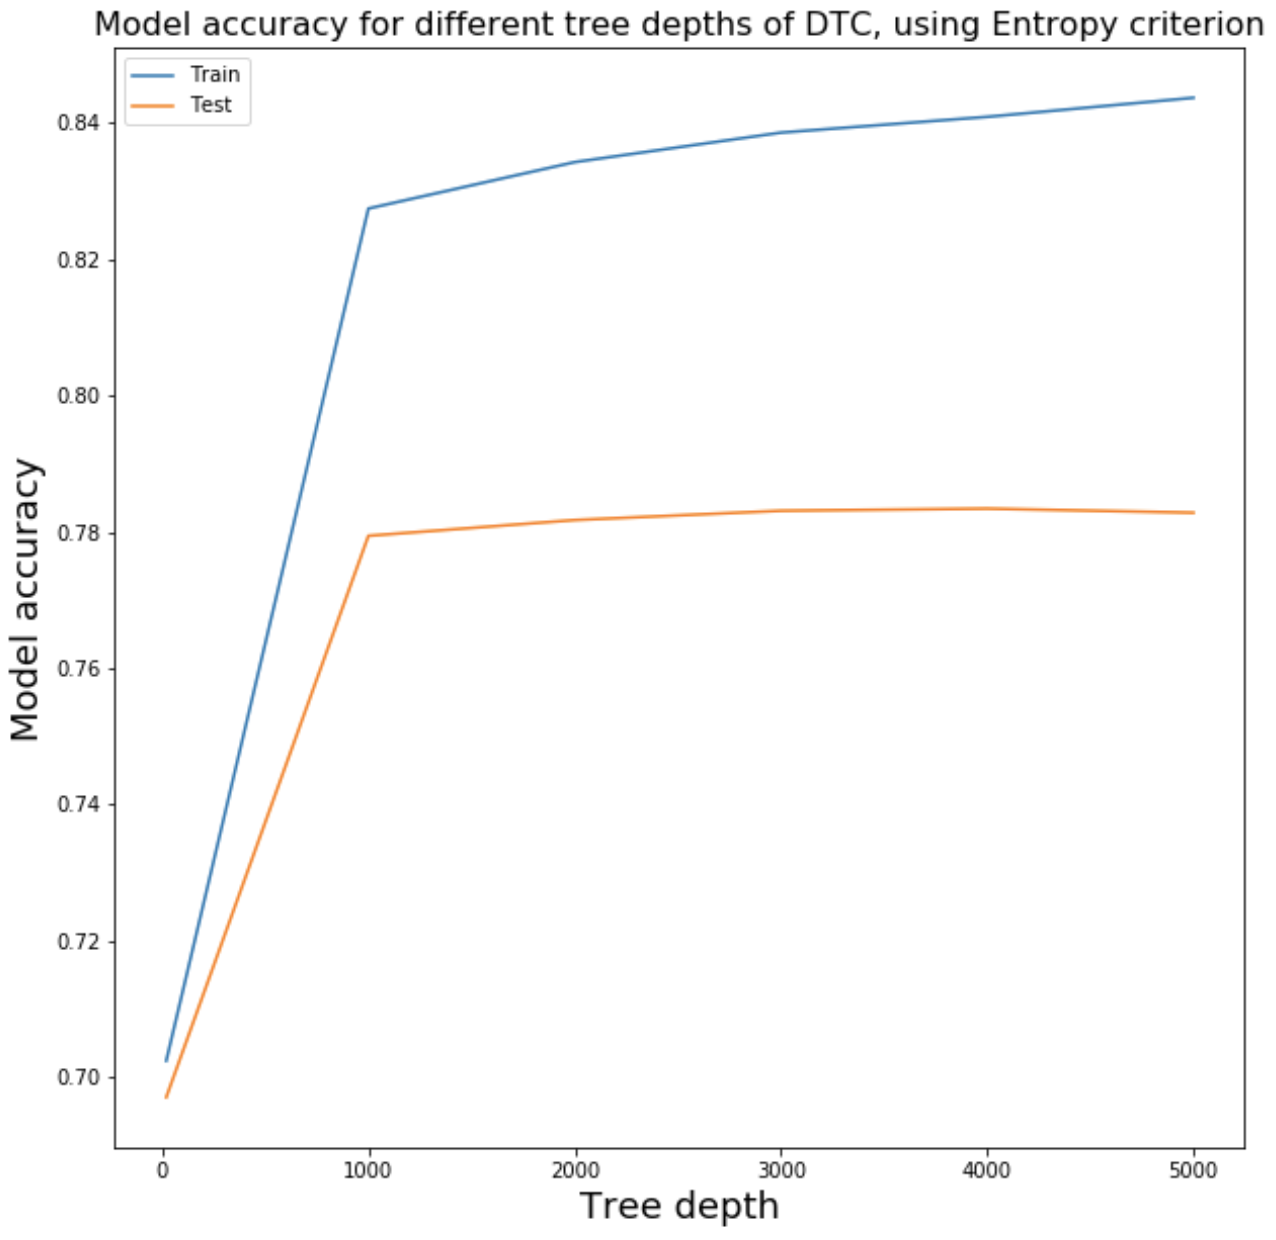
\includegraphics[scale=0.5]{Figure_4_DTC_depths_20_5000_Entropy.png}
\caption{Model accuracy curve with different depth, using Entropy criterion.}
\label{Figure:DTC_depth_20_5000_entropy}
\end{figure}

\begin{table}[h]
\centering
\begin{tabular}{ | c || c | c | c | c | c | c |}
\hline
\textbf{ Tree depth } & \text{ 20 } & \text{ 1000 } & \text{ 2000 } & \text{ 3000 }  & \text{ 4000 } & \text{ 5000 } \\
\hline
\textbf{ Accuracy } & \text{ 0.6971 } & \text{ 0.7794 } & \text{ 0.7817 } & \text{ 0.7831 }  & \text{ 0.7834 } & \text{ 0.7828 }\\
\hline
\end{tabular}
\caption{DTC prediction accuracies on test set with different tree depths, using Entropy criterion. }
\label{table:DTC_accuracy_depth_20_5000_entropy}
\end{table}

\noindent
The results are shown in Figure~\ref{Figure:DTC_depth_20_5000_entropy}  and Table~\ref{table:DTC_accuracy_depth_20_5000_entropy}. It turns out that the Entropy model shares a very similar trend to the Gini Impurity model as oth models achieved around 78\% accuracy at depths 1000.

\section{Support vector machine}
Support Vector Machine (SVM) is another powerful ML algorithm that can train classification models. The details of its underlying working mechanisms are not discussed in this project. More reading on how it is implemented can be found \href{https://en.wikipedia.org/wiki/Support-vector_machine}{\textbf{here}}. The purpose of using this algorithm is to compare the performance of different ML models when tasked with sentiment analysis. More precisely, sentiment analysis of the reviews which this analyser system is based on.

\subsubsection{Parameters}
In order to find the best model, there are many configurable parameters associated with the SVM algorithm. The main function used for this section is the \code{sklearn.svm.SVC()} function from the Scikit-Learn package. According to its official documentation, which can be found in this \href{https://scikit-learn.org/stable/modules/generated/sklearn.svm.SVC.html#sklearn.svm.SVC}{\textbf{link}}, there is a list of configurable parameters. For the development of this project, only the following list of parameters will be configured:

\begin{itemize}
	\item \(C\) the regularisation parameter.
	\item \(Kernel\)
	\item \(Gamma\)
\end{itemize}

\subsubsection{K-Fold Cross Validation}
Cross validation is a technique used when training ML models. It helps to resolve the problem of having only a limited amount of data. As for this project, the dataset is obtained directly from  \url{kaggle.com}. Thus the number of data samples available are fixed. To make the best out of the data, cross validation is introduced in this section.
\\\\
Cross validation works by training several machine learning models on subsets of the data and validate their performance on the complementary sets of the data. For example, the dataset can be divided into 4 subsets, used to train 4 different models. Model 1 uses the first 25\% of the first subset for evaluation, and the rest 75\% for training. The second model will use the second 25\% of the second subset of data for evaluation, and so on. A more intuitive representation is shown in Figure~\ref{Figure:cross_validation}.\\

\begin{figure}[h]
\centering
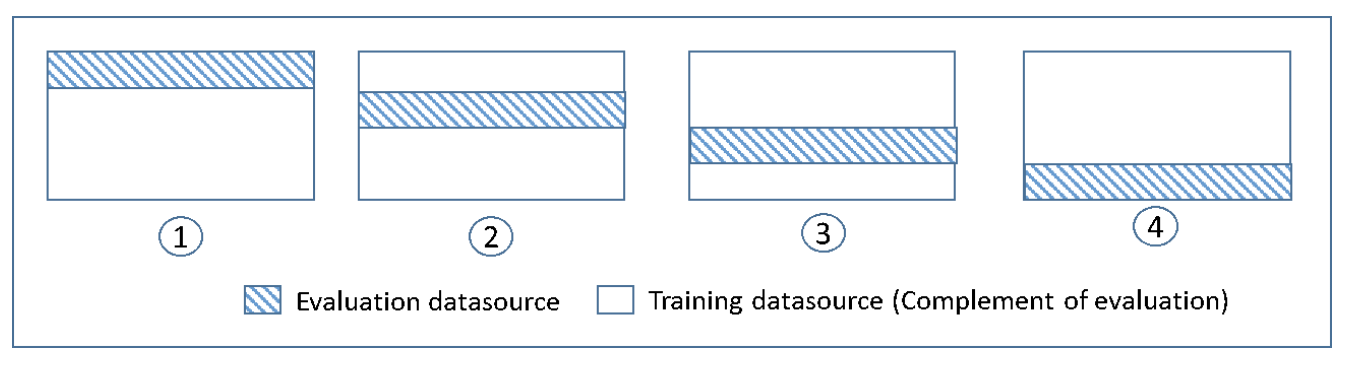
\includegraphics[scale=0.5]{cross_validation.png}
\caption{Example illustration of 4-fold cross validation.}
\label{Figure:cross_validation}
\end{figure}

A more advanced version of cross validation is K-Fold Cross Validation. The input data is split into k subsets, a model can be trained on all but one of the subsets, and use the last subset for evaluation. This process can be repeated for K times, each time using a different subset for evaluation. Thus all of the data samples will be used in training, the model produced will less likely to underfit the data.

\subsubsection{Testing using GridSearchCV}
The number of different parameters, together with K-fold cross validation can be cumbersome to implement. A useful tool provided by the Scikit-Learn package is the sklearn.model\_selection. GridSearchCV() function. It takes a set of parameters to be configured and performs an exhaustive search over the different combinations to find the best parameters for a model.
\\\\
After undergoing the exhaustive search, the best parameters found are displayed in Table~\ref{table:SVC_parameters}. The evaluation metric results are shown in Table

\begin{table}[h]
\centering
\begin{tabular}{ | c | c | c |}
\hline
\text{ \textbf{C}: 1 }  & \text{ \textbf{Gamma}: 1 } & \text{ \textbf{Kernel}: `rbf' } \\
\hline
\end{tabular}
\caption{Best parameters for SVC using GridSearchCV().}
\label{table:SVC_parameters}
\end{table}

\begin{table}[h!]
\centering
\begin{tabular}{  c | c | c | c |}
\cline{2-4}
&  \textbf { precision } &  \textbf  { recall } & \textbf  { f1-score }  \\
\hline
\multicolumn{1}{|c|}{ \textbf {0}} & 0.74 & 0.83 & 0.78 \\
\hline
\multicolumn{1}{|c|}{ \textbf {1}} & 0.81 & 0.72 & 0.76 \\
\hline
\hline
\multicolumn{1}{|c|}{ \textbf {Accuracy}} & \multicolumn{3}{|c|}{0.7715} \\
\hline
\end{tabular}
\caption{Evaluation metric of the SVC classifier with the best parameters.}
\label{table:SVC_performance}
\end{table}

\section{Random Forest Classifier}
Random Forest Classifier (RFC) is an even more powerful tree based classifier than the DTC. When training a model, this algorithm produces many different tree classifiers, and the trees work collectively in when making the final predictions. 
\\\\
There are 4 main steps of the Random Forest Classifier:

\begin{enumerate}
	\item Select random samples from a given dataset.
	\item Construct a decision tree for each sample and get a prediction result from each decision tree.
	\item Perform a vote for each predicted result.
	\item Select the prediction result with the most votes as the final prediction.
\end{enumerate}


\subsubsection{Performance result}
In Table~\ref{table:RFC_performance} is the evaluation metric of the RFC using a max depth of 1000.

\begin{table}[h!]
\centering
\begin{tabular}{  c | c | c | c |}
\cline{2-4}
&  \textbf { precision } &  \textbf  { recall } & \textbf  { f1-score }  \\
\hline
\multicolumn{1}{|c|}{ \textbf {0}} & 0.75 & 0.81 & 0.77 \\
\hline
\multicolumn{1}{|c|}{ \textbf {1}} & 0.79 & 0.73 & 0.76 \\
\hline
\hline
\multicolumn{1}{|c|}{ \textbf {Accuracy}} & \multicolumn{3}{|c|}{0.7678} \\
\hline
\end{tabular}
\caption{Evaluation metric of the RFC classifier.}
\label{table:RFC_performance}
\end{table}

\section{MLP Classifier}
“MLPClassifier stands for Multi-layer Perceptron classifier which in the name itself connects to a Neural Network. Unlike other classification algorithms such as Support Vectors or Naive Bayes Classifier, MLPClassifier relies on an underlying Neural Network to perform the task of classification." For the implementation of this classifier, the \code{sklearn.neural\_network.MLPClassifier()} function from the Scikit-Learn package is used. [9]

\subsubsection{Testing using GridSearchCV}
Below is the list of parameters being configured using the \code{sklearn.model\_selection.GridSearchCV()} function:

\begin{itemize}
	\item \code{hidden\_layer\_sizes}
	\item \code{activation}
	\item \code{solver}
	\item \code{alpha}
	\item \code{learning\_rate}
\end{itemize}

\subsubsection{Performance result}
The final results of the MLP classifier model generated is recorded in Table~\ref{table:MLP_performance}. 

\begin{table}[h!]
\centering
\begin{tabular}{  c | c | c | c |}
\cline{2-4}
&  \textbf { precision } &  \textbf  { recall } & \textbf  { f1-score }  \\
\hline
\multicolumn{1}{|c|}{ \textbf {0}} & 0.76 & 0.82 & 0.79 \\
\hline
\multicolumn{1}{|c|}{ \textbf {1}} & 0.81 & 0.75 & 0.78 \\
\hline
\hline
\multicolumn{1}{|c|}{ \textbf {Accuracy}} & \multicolumn{3}{|c|}{0.7845} \\
\hline
\end{tabular}
\caption{Evaluation metric of the MLP classifier.}
\label{table:MLP_performance}
\end{table}

\section{Model Selection}
The best performance of the different models generated in the previous sections are compared in Table~\ref{table:model_comparisons}. Other property comparisons are illustrated in Figure~\ref{Figure:Evaluation_metrix_barhz}.
\\
\begin{table}[h]
\centering
\begin{tabular}{ | c || c | c | c | c |}
\hline
\textbf{ Classifiers } & \text{ DTC-1000 } & \text{ SVM } & \text{ RFC } & \text{ MLPClassifier } \\
\hline
\textbf{ Accuracy } & \text{ 0.7807 } & \text{ 0.7715 } & \text{ 0.7678 } & \text{ 0.7845 } \\
\hline
\end{tabular}
\caption{Accuracy comparison between different models. }
\label{table:model_comparisons}
\end{table}

\begin{figure}[h]
\centering
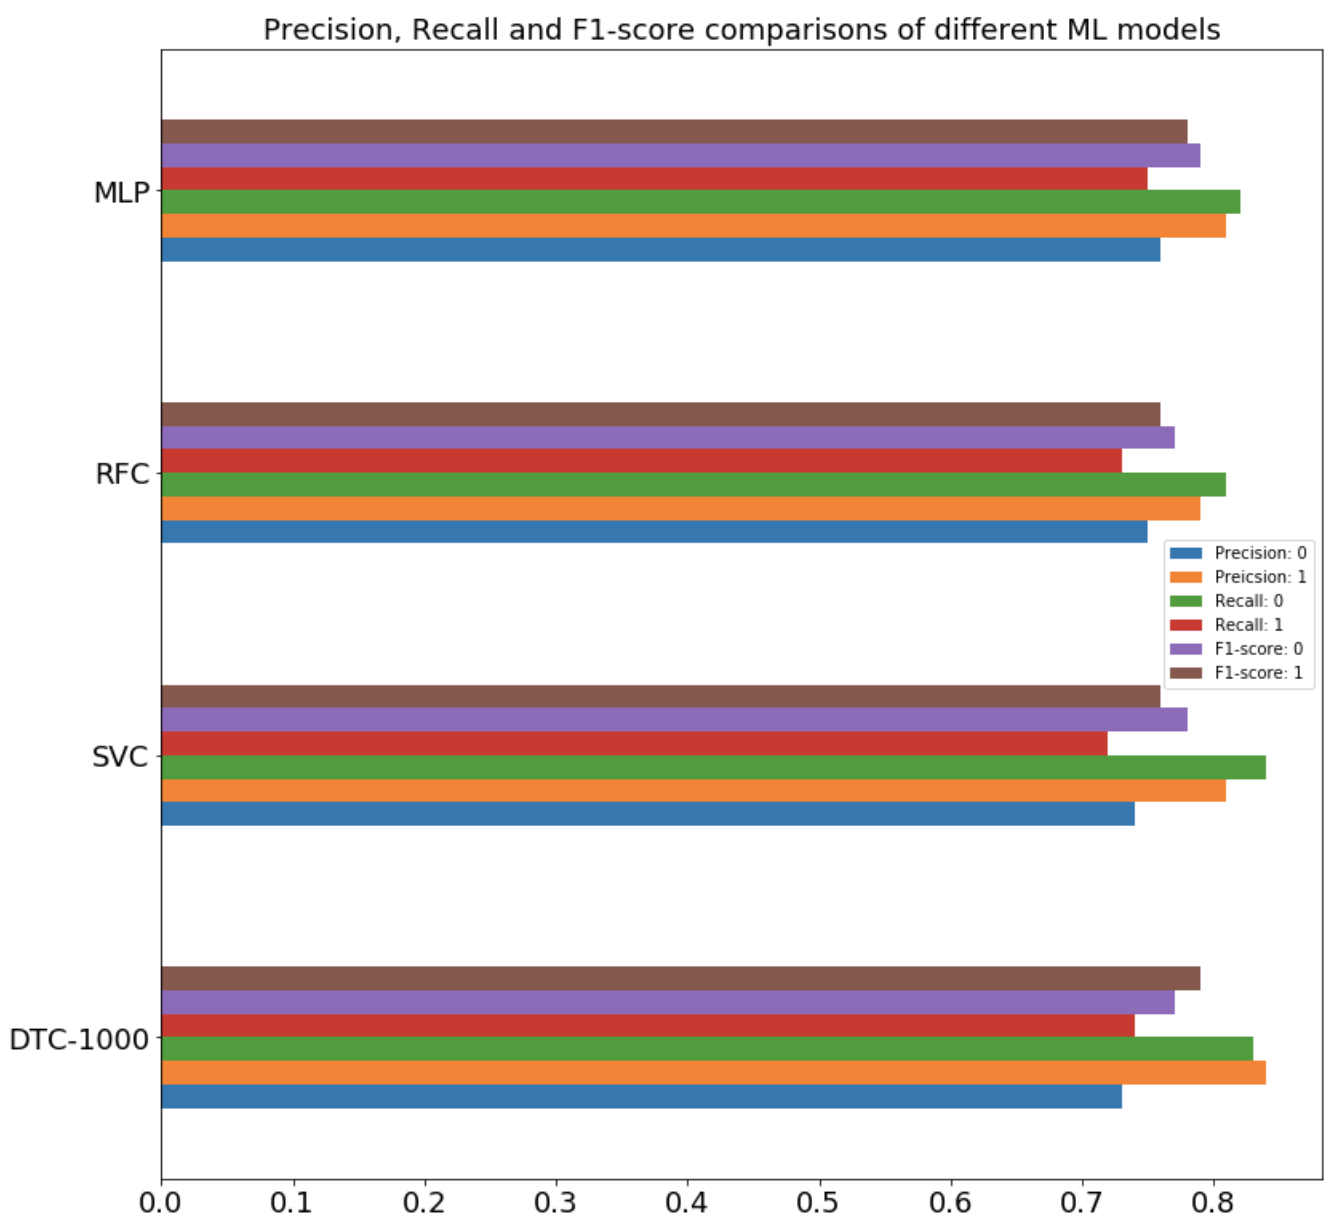
\includegraphics[scale=0.6]{Evaluation_metrix_barhz.png}
\caption{Bar chart of the evaluation metrics comparisons.}
\label{Figure:Evaluation_metrix_barhz}
\end{figure}

\subsubsection{Bagging}
As seen from Figure~\ref{Figure:Evaluation_metrix_barhz}, all the models have very similar performances in terms of accuracy and the various precision and recall values. The high scores achieved suggesting they are all equally reliable models that can be used in the sentiment analysis of this review analyser syste. Therefore the approach taken in this project is to create a model ensemble, also called “bagging", where all 4 models are used to produce the final prediction. This is similar to the working mechanism of the Random Forest Classifier, for every input review, its sentiment will be predicted by each of the four models, and the sentiment with the most vote will become final output. This further improves the reliability of the sentiment analysis, which in turn improves the confidence of the system in selecting the best and worst features of each hotel.



\chapter{Conclusions and Evaluation}
\section{Achievements}
There are three key topics achieved in this project. The first one being best and worst features extraction from the hotel reviews. Second one is sentiment analysis on the textual data. Third one is hotel report generation with user accessible interface. 

\subsubsection{Best and worst features extraction}
Based on the “Hotel\_Reviews.csv" dataset from the \href{https://www.kaggle.com/jiashenliu/515k-hotel-reviews-data-in-europe}{\textbf{kaggle}} website, a thorough analysis on the textual data has been carried out. This project seeks to incorporate various NLP techniques such as lexical, syntactic and semantic analysis to stratify long strings of data into smaller and more meaningful chunks. This allows hotel feature extractions to be more accurate, at the same time the corresponding values that describes the features were also captured by the system. Thus the end results are more understandable and interesting to the users.

\subsubsection{Sentiment analysis}
As mentioned in the earlier chapters, the motivation for sentiment analysis comes from mixed sentiments in reviews. In some negative reviews, the users may have been talking about some aspects of the hotel which they liked, and vice versa talking about the downsides in their positive comments. Hence by digging deeper into each reviews and transform the textual data into numerical representations using TF-IDF  has allowed sentiment analysis to become possible in this project. Four different ML models have been trained with high accuracy in classifying the sentiment of reviews in the dataset. The strengths of these models are combined using the “bagging" technique to further strengthen the prediction of sentiments. Hence the mixed sentences in reviews can be reclassified, producing better feature extractions by the system.

\subsubsection{User accessible interface}
The majority of the heavy contents lies in the implementation of data processing and NLP, which are essential to forming a reliable backend database. However, the processed data are worthless if they cannot be utilised. Thus another main area of focus in the development of this system is building an accessible user interface. This project has used the Django web framework to build a user facing front-end and a MVT server as the back-end. Upon receiving a user request, the back-end server fetches the processed data from the database to generate the requested report and renders it on the user's web browser. This therefore brings all the separate components together, making the system complete.

\section{Challenges and Evaluation}
\subsubsection{Defining grammar}
One of the challenges faced in this project is in the syntactic analysis stage. How to solve the problem of chunking was not immediately apparent. Various experiments have been carried out, such as extracting words within a certain distances from each other, perform Tf-IDF on raw reviews to identify the most used words. However the “features" extracted were noisy and less interpretable. Better progress was made with the realisation of finding noun phrases within the sentences. Then after knowing which parts of the reviews to extract, it became much clearer that some forms of matching to the POS-tags of the word tokens are required. The new challenge faced then was to devise the appropriate grammars for chunking. The breakthrough was in using regular expression to capture variations of the noun phrases, rather than using many predefined grammars that tries to capture the different sentence structures. However, after constructing a grammar that works well in chunking the positive reviews, it produced poor results when tested against the negative reviews. The reason behind is that in negative reviews, the sentences in the string tends to be longer, which makes it difficult to properly perform chunking. For a long string, multiple chunks can be captured at the same time with some degree of overlapping. Some words from the previous sentence might be thought to have a connection with the words in the second sentence. Therefore, it is necessary to separate the raw review from into separate sentences first to reduce ambiguity. The two approaches taken are using regular expressions and \code{sent\_tokenize()} function from the NLTK package to automatically separate individual sentences in a review.
\\\\
Positive reviews are easier to process, because reviewers tends to be in a more relaxed state. The good aspects about a certain feature are simply stated. The negative reviews on the other hand are more strenuous to deal with because they tend to be longer than the positve review. The context described is also more complicated because reviewers are most likely to be more impulsive when expressing why they disliked certain aspects about the hotel. Also the wording are not as straightforward, for example, a broken TV may be written as "TV was broken", or "TV did not work". If only ``work" is matched by the grammar, and the negator ``not" is not, then it changes the meaning of the sentence entirely. 

\subsubsection{ML models}
Another challenging aspect arises from the ML models. The ease of training a model using the Scikit-Learn package can easily make the sentiment analysis problem look easier than it is. Underestimating the task often led to overfitting models that does not perform well in the real application. Therefore it is important to do background readings around the topic and understand how the parameters of the models should be configured, and knowing how to evaluate the performance.
\\\\
After having successfully trained the 4 models that performs equally well, choosing which model to be used by the system required some considerations. The inspiration of using the “bagging" method came from the paper written by Pedro Domingos. In the paper he suggested “creating a model ensembles is now standard. In the simplest technique, called \(bagging\), we simply generate random variations of the training set by resampling, learn a classifier on each, and combine the results by voting. This works because it greatly reduces variance while only slightly increasing bias." Hence, a voting system that ensembles the 4 different classifiers were used in the sentiment analysis of this project.
\\\\
There are already many sentiment analysers available on the internet, even within the NLTK package, there exist a \code{nltk.sentiment.sentiment\_analyzer.SentimentAnalyzer()} function which can be simply imported and used. However, one of the decisions made in the development of this system was to train a dedicated sentiment classifier based on the dataset. This is because the models would be fitted better to the dataset, in particular reviews from Booking.com. Thus is capable of determining sentiments of future reviews.



\section{Future Work}
In sentiment analysis, training data can be further improved by taking into account other factors such as polarity, negator and modifier. This will require a more complex grammar being defined to capture more information from the negative reviews. The advantage would be that sentences such as "the room was not so clean" can be mapped by the grammar, values such as "not clean" can be extracted. This could increase the precision of the models correctly classifying reviews with negative sentiment. [10]
\\\\
Overall, the negative reviews are more complexed to process. For future work, maybe instead of using the results from the text analysis, which relies on POS-tags, use the raw forms of the reviews, and prepare the training data with N-gram approach, maximise the chance of the system identifying the main focus of the review. Therefore, the system may be modified by training a classifier for positive reviews, and a classifier for negative negative reviews. So when reclassifying the individual sentences, they need to be examined by the positive and negative classifier, then the class with the highest confidence in its prediction will be used. This is down to the competition between the model precision scores of the positive and negative classifiers, which may produce a more robust result.
\\\\
Instead of using various \code{.csv} files as the back-end database of the system, the processed files could be transformed into a MySql database. That way the data stored are more maintainable and scalable. The speed to fetching data and responding to user request can also be optimised.




%\chapter{Bibliography}
%
%%\begin{thebibliography}{HHM99}
%%
%%\end{thebibliography}
%
%[1] “515K Hotel Reviews Data in Europe", Kaggle.com, 2021. [Online]. Available: \url{https://www.kaggle.com/jiashenliu/515k-hotel-reviews-data-in-europe}. [Accessed: 07- Nov- 2020].
%
%[2] T. Barrus, "pyspellchecker", PyPI, 2021. [Online]. Available: \url{https://pypi.org/project/pyspellchecker}. [Accessed: 14- Dec- 2020].
%
%[3] “Inflection - Wikipedia", En.wikipedia.org, 2021. [Online]. Available: \url{https://en.wikipedia.org/w/index.php?title=Inflection&oldid=1016909335}. [Accessed: 06- Jan- 2021].
%
%[4] B. Stecanella, "What is TF-IDF?", Monkeylearn.com, 2019. [Online]. Available: \url{https://monkeylearn.com/blog/what-is-tf-idf/#:~:text=TF%2DIDF%20enables%20us%20to,in%20a%20machine%20learning%20algorithm}. [Accessed: 20- Dec- 2020].
%
%[5] “Classification: Precision and Recall  |  Machine Learning Crash Course", Google Developers, 2020. [Online]. Available: \url{https://developers.google.com/machine-learning/crash-course/classification/precision-and-recall}. [Accessed: 06- Feb- 2021].
%
%[6]Y. Sakkaf, "Decision Trees for Classification: ID3 Algorithm Explained", Medium, 2021. [Online]. Available: https://towardsdatascience.com/decision-trees-for-classification-id3-algorithm-explained-89df76e72df1. [Accessed: 31- Mar- 2021].
%
%[7]"Cross-Validation - Amazon Machine Learning", Docs.aws.amazon.com, 2021. [Online]. Available: https://docs.aws.amazon.com/machine-learning/latest/dg/cross-validation.html. [Accessed: 15- Mar- 2021].
%
%[8]A. Navlani, "Understanding Random Forests Classifiers in Python", Datacamp, 2018. [Online]. Available: https://www.datacamp.com/community/tutorials/random-forests-classifier-python. [Accessed: 09- Mar- 2021].
%
%[9]A. Nair, "A Beginner’s Guide To Scikit-Learn’s MLPClassifier", Analytics India Magazine, 2019. [Online]. Available: \url{https://analyticsindiamag.com/a-beginners-guide-to-scikit-learns-mlpclassifier/#:~:text=MLPClassifier%20stands%20for%20Multi%2Dlayer,perform%20the%20task%20of%20classification}. [Accessed: 26- Mar- 2021].
%
%[10]"Sentiment entries | MeaningCloud", Meaningcloud.com. [Online]. Available: https://www.meaningcloud.com/developer/resources/doc/sentiment-models/entries. [Accessed: 06- Apr- 2021].

\appendix

\chapter{Code}
Link to source code: \url{https://github.com/1109LLL/FYP.git}

\begin{lstlisting}[language=Python,label={lst:lexical},caption={Lexical Analysis} ]
    # Lexical analysis
    def lexical_analysis(self,sent):
        # Tokenising the sentence into separate word tokens
        sent = sent.lower()
        tokenise = word_tokenize(sent)

        # Check spelling
        tokenise = self.spell_check(tokenise)

        # Apply parts of speech tags to the tokens
        pos_tagged = nltk.pos_tag(tokenise)
        return pos_tagged
    
    def spell_check(self, tokens):
        spell = SpellChecker()
        misspelled = spell.unknown(tokens)

        for word in misspelled:
            tokens[tokens.index(word)] = spell.correction(word)
        return tokens

\end{lstlisting}


\begin{lstlisting}[language=Python,label={lst:POS-tag},caption={POS Tags} ]
'''
POS tags list
TAG	 POS	MORPHOLOGY	DESCRIPTION
$	SYM		symbol, currency
``	PUNCT	PunctType=quot PunctSide=ini	opening quotation mark
''	PUNCT	PunctType=quot PunctSide=fin	closing quotation mark
,	PUNCT	PunctType=comm	punctuation mark, comma
-LRB-	PUNCT	PunctType=brck PunctSide=ini	left round bracket
-RRB-	PUNCT	PunctType=brck PunctSide=fin	right round bracket
.	PUNCT	PunctType=peri	punctuation mark, sentence closer
:	PUNCT		punctuation mark, colon or ellipsis
ADD	X		email
AFX	ADJ	Hyph=yes	affix
CC	CCONJ	ConjType=comp	conjunction, coordinating
CD	NUM	NumType=card	cardinal number
DT	DET		determiner
EX	PRON	AdvType=ex	existential there
FW	X	Foreign=yes	foreign word
GW	X		additional word in multi-word expression
HYPH	PUNCT	PunctType=dash	punctuation mark, hyphen
IN	ADP		conjunction, subordinating or preposition
JJ	ADJ	Degree=pos	adjective
JJR	ADJ	Degree=comp	adjective, comparative
JJS	ADJ	Degree=sup	adjective, superlative
LS	X	NumType=ord	list item marker
MD	VERB	VerbType=mod	verb, modal auxiliary
NFP	PUNCT		superfluous punctuation
NIL	X		missing tag
NN	NOUN	Number=sing	noun, singular or mass
NNP	PROPN	NounType=prop Number=sing	noun, proper singular
NNPS	PROPN	NounType=prop Number=plur	noun, proper plural
NNS	NOUN	Number=plur	noun, plural
PDT	DET		predeterminer
POS	PART	Poss=yes	possessive ending
PRP	PRON	PronType=prs	pronoun, personal
PRP$	DET	PronType=prs Poss=yes	pronoun, possessive
RB	ADV	Degree=pos	adverb
RBR	ADV	Degree=comp	adverb, comparative
RBS	ADV	Degree=sup	adverb, superlative
RP	ADP		adverb, particle
SP	SPACE		space
SYM	SYM		symbol
TO	PART	PartType=inf VerbForm=inf	infinitival "to"
UH	INTJ		interjection
VB	VERB	VerbForm=inf	verb, base form
VBD	VERB	VerbForm=fin Tense=past	verb, past tense
VBG	VERB	VerbForm=part Tense=pres Aspect=prog	verb, gerund or present participle
VBN	VERB	VerbForm=part Tense=past Aspect=perf	verb, past participle
VBP	VERB	VerbForm=fin Tense=pres	verb, non-3rd person singular present
VBZ	VERB	VerbForm=fin Tense=pres Number=sing Person=three	verb, 3rd person singular present
WDT	DET		wh-determiner
WP	PRON		wh-pronoun, personal
WP$	DET	Poss=yes	wh-pronoun, possessive
WRB	ADV		wh-adverb
XX	X		unknown
_SP	SPACE	

src = https://spacy.io/api/annotation
'''
\end{lstlisting}

\begin{lstlisting}[language=Python,label={lst:grammar_chunking},caption={Grammars used for chunking in reviews in Syntactic Analysis.} ]
    # Syntactic Analysis
    def syntactic_analysis_for_positives(self,sent):
        # Define chunking grammar using regular expression
        # grammar_1 captures sentence structure where the adjectives comes after the nouns
        grammar_1 = r"""
                    NP: {(<NN>|<NNS>)+<PRP>*<VBD>*<VBZ>*<RB>*<VBN>*<JJ>*((<CC><VBD>+)|(<CC><RB>+<JJ>*)|(<CC><VBN>+)|(<CC><JJ>+))*}
                    """
        # grammar_2 captures sentence structure where the adjectives comes before the nouns
        grammar_2 = r"""
                    NP: {<JJ>(<NN>|<NNS>)+}
                    """

        chunks_1 = self.grammar_parsing(grammar_1,sent)
        chunks_2 = self.grammar_parsing(grammar_2,sent)
        chunks = chunks_1 + chunks_2

        return chunks
    
    def syntactic_analysis_for_negatives(self, sent):
        # Define chunking grammar using regular expression
        
        grammar_1 = r"""
                    NP: {(<JJ>|<RB>|<VBD>)(<NN>|<NNS>)}
                    """
        # grammar_2 captures sentence structure where the adjectives comes after the nouns
        grammar_2 = r"""
                    NP: {(<NN>|<NNS>)<VBP>*<VBD>*<JJ>*<VB>*}
                    """
        
        chunks_1 = self.grammar_parsing(grammar_1,sent)
        chunks_2 = self.grammar_parsing(grammar_2,sent)
        chunks = chunks_1 + chunks_2

        return chunks
    
    # Parse the sentence and chunking using grammar
    def grammar_parsing(self,grammar,sent):
        cp = nltk.RegexpParser(grammar)
        result = cp.parse(sent)

        chunks = []
        for subtree in result.subtrees():
            # if subtree length smaller than 2 -> single words -> ignore
            if len(subtree) < 2 or subtree.label()=="S":
                continue

            # Check for duplicates
            if not subtree in chunks:
                chunks.append(subtree)

        return chunks
\end{lstlisting}

\begin{lstlisting}[language=Python,label={lst:tfidf},caption={Document term matrix using TF-IDF.} ]
    def form_training_set_for_sentiment_clf_decision_tree(self):
        getter = Getter()
        hotel_list = getter.getHotelList()

        pos_val = []
        neg_val = []
        # Extract the positive and negative dictionaries (noun and adj) from each hotel
        # obtain a list of only the values
        for hotel in hotel_list.values:
            hotel_name = hotel[0]

            pos_dict = getter.get_pos_noun_adj_dict_of_hotel(hotel_name)
            pos_values_list = list(pos_dict.values())
            for value in pos_values_list:
                if len(value) == 1:
                    pos_val.append(value[0])
                else:
                    pos_val.append(' '.join(value))


            neg_dict = getter.get_neg_noun_adj_dict_of_hotel(hotel_name)
            neg_values_list = list(neg_dict.values())
            for value_ in neg_values_list:
                if len(value_) == 1:
                    neg_val.append(value_[0])
                else:
                    neg_val.append(' '.join(value_))

        y_pos_label = [1] * len(pos_val)
        y_neg_label = [0] * len(neg_val)    
        
        X = pos_val + neg_val
        y = y_pos_label + y_neg_label

        return X, y

    def fit_training_set_using_tfidf_vectorizer(self):
        print("------------------------------------------")
        now = datetime.datetime.now()
        print("{} : start fitting tfidf".format(now.strftime("%Y-%m-%d %H:%M:%S")))

        getter = Getter()
        X, y = getter.get_training_set_for_sentiment_clf_decision_tree()
        
        tfIdfVectorizer = TfidfVectorizer(use_idf=True)
        X_tfidf = tfIdfVectorizer.fit_transform(X)

        now = datetime.datetime.now()
        print("{} : finished fit_transform".format(now.strftime("%Y-%m-%d %H:%M:%S")))
        print("------------------------------------------")

        return X_tfidf, tfIdfVectorizer
\end{lstlisting}
\begin{lstlisting}[language=Python,label={lst:GridSearchCV},caption={GridSearchCV to find best SVC classifier.} ]
print("------------------------------------------")
now = datetime.datetime.now()
print("{} : start training".format(now.strftime("%Y-%m-%d %H:%M:%S")))

getter = Getter()
X_tfidf, y, tfIdfVectorizer = getter.get_X_tfidf_y_training_set_for_sentiment_clf_decision_tree()

# Split dataset into training set and test set
X_train, X_test, y_train, y_test = train_test_split(X_tfidf, y, test_size=0.2, random_state=42)

# Create SVC object
svc = SVC(random_state=42)

# Train Decision Tree Classifer
svc = svc.fit(X_train,y_train)

param_grid = {'C': [0.1, 1, 10, 100, 1000], 
              'gamma': [1, 0.1, 0.01, 0.001, 0.0001],
              'kernel': ['rbf', 'poly']} 

grid = GridSearchCV(SVC(), param_grid, cv=5, refit = True, verbose = 3, n_jobs=-1)
  
# fitting the model for grid search
grid.fit(X_train, y_train)

now = datetime.datetime.now()

# Create predictions

print("best estimator = {}".format(grid.best_estimator_))
print("best parameters = {}".format(grid.best_params_))

grid_predictions = grid.predict(X_test)


# Model Accuracy
print(metrics.classification_report(y_test,grid_predictions))
print("Accuracy: {}".format(round(metrics.accuracy_score(y_test, grid_predictions),4)))
print("-------------------------------------")
\end{lstlisting}

\end{document}